\documentclass[a4paper,10pt,oneside]{article}
\usepackage[utf8]{inputenc}
\usepackage[usenames,dvipsnames]{color}
\usepackage[usenames,dvipsnames]{xcolor}
\usepackage[english,russian]{babel} 
\usepackage{tikz}


\oddsidemargin=0pt
\textwidth=165mm

\author{Соколов Николай, ФПКиФ 2-2}
\title{Лабораторная работа по операционным\nolinebreak{} системам. \linebreak
Алгоритмы планирования ввода-вывода. Алгоритм C-LOOK.}
\date{}

\begin{document}
\maketitle

\section{Общие сведения}
Программа представляет собой реализацию некоторых алгоритмов планирования ввода-вывода, таких как:
\begin{itemize}
 \item First Come First Served (FCFS)
 \item Shortest Seek Time First (SSTF)
 \item SCAN
 \item C-SCAN
 \item LOOK
 \item C-LOOK
\end{itemize}
Реализация выполнена на языке \textit{C++} с использованием кроссплатформенного фреймворка \textit{Qt} и может быть скомпилирована под большинство
современных платформ, таких как \textit{Windows}, \textit{GNU/Linux}, \textit{MacOS X}, а так же \textit{Maemo} и \textit{Symbian}. 
Для функционирования программы необходимы библиотеки \textit{QtCore} и \textit{QtGUI}.

\section{Функциональное назначение}
По введенной последовательности цилиндров программа формирует правильную очередность чтения данных с диска в соответствии с выбранным алгоритмом
и направлением движения головки жесткого диска. Кроме этого, в окне программы отображается схематическое анимированное изображение жесткого диска,
на котором наглядно иллюстрируется полученная последовательность чтения секторов.

\section{Описание логической структуры}
Объектная структура состоит из двух классов: \texttt{Widget}, реализующего окно, и \texttt{HddWidget}, реализующего виджет жесткого диска. Классы объявлены в файлах
\texttt{widget.h} и \texttt{hddwidget.c} соответственно. Объектная структура приведена на следующей UML диаграмме:

% Graphic for TeX using PGF
% Title: /home/chemikadze/programming/qt/ioshed/article/classes.dia
% Creator: Dia v0.97.1
% CreationDate: Mon May  3 22:58:56 2010
% For: chemikadze
% \usepackage{tikz}
% The following commands are not supported in PSTricks at present
% We define them conditionally, so when they are implemented,
% this pgf file will use them.
\ifx\du\undefined
  \newlength{\du}
\fi
\setlength{\du}{14.5\unitlength}
\begin{tikzpicture}
\pgftransformxscale{1.000000}
\pgftransformyscale{-1.000000}
\definecolor{dialinecolor}{rgb}{0.000000, 0.000000, 0.000000}
\pgfsetstrokecolor{dialinecolor}
\definecolor{dialinecolor}{rgb}{1.000000, 1.000000, 1.000000}
\pgfsetfillcolor{dialinecolor}
\pgfsetlinewidth{0.100000\du}
\pgfsetdash{}{0pt}
\definecolor{dialinecolor}{rgb}{1.000000, 1.000000, 1.000000}
\pgfsetfillcolor{dialinecolor}
\fill (2.100000\du,0.100000\du)--(2.100000\du,1.500000\du)--(16.847500\du,1.500000\du)--(16.847500\du,0.100000\du)--cycle;
\definecolor{dialinecolor}{rgb}{0.000000, 0.000000, 0.000000}
\pgfsetstrokecolor{dialinecolor}
\draw (2.100000\du,0.100000\du)--(2.100000\du,1.500000\du)--(16.847500\du,1.500000\du)--(16.847500\du,0.100000\du)--cycle;
% setfont left to latex
\definecolor{dialinecolor}{rgb}{0.000000, 0.000000, 0.000000}
\pgfsetstrokecolor{dialinecolor}
\node at (9.473750\du,1.050000\du){Widget};
\definecolor{dialinecolor}{rgb}{1.000000, 1.000000, 1.000000}
\pgfsetfillcolor{dialinecolor}
\fill (2.100000\du,1.500000\du)--(2.100000\du,8.650000\du)--(16.847500\du,8.650000\du)--(16.847500\du,1.500000\du)--cycle;
\definecolor{dialinecolor}{rgb}{0.000000, 0.000000, 0.000000}
\pgfsetstrokecolor{dialinecolor}
\draw (2.100000\du,1.500000\du)--(2.100000\du,8.650000\du)--(16.847500\du,8.650000\du)--(16.847500\du,1.500000\du)--cycle;
% setfont left to latex
\definecolor{dialinecolor}{rgb}{0.000000, 0.000000, 0.000000}
\pgfsetstrokecolor{dialinecolor}
\node[anchor=west] at (2.250000\du,2.200000\du){-m\_queries: QVector <int>};
% setfont left to latex
\definecolor{dialinecolor}{rgb}{0.000000, 0.000000, 0.000000}
\pgfsetstrokecolor{dialinecolor}
\node[anchor=west] at (2.250000\du,2.925000\du){Запросы чтения};
% setfont left to latex
\definecolor{dialinecolor}{rgb}{0.000000, 0.000000, 0.000000}
\pgfsetstrokecolor{dialinecolor}
\node[anchor=west] at (2.250000\du,4.050000\du){-m\_moveCount: int};
% setfont left to latex
\definecolor{dialinecolor}{rgb}{0.000000, 0.000000, 0.000000}
\pgfsetstrokecolor{dialinecolor}
\node[anchor=west] at (2.250000\du,4.775000\du){Счетчик шагов};
% setfont left to latex
\definecolor{dialinecolor}{rgb}{0.000000, 0.000000, 0.000000}
\pgfsetstrokecolor{dialinecolor}
\node[anchor=west] at (2.250000\du,5.900000\du){-ui: Ui::Widget};
% setfont left to latex
\definecolor{dialinecolor}{rgb}{0.000000, 0.000000, 0.000000}
\pgfsetstrokecolor{dialinecolor}
\node[anchor=west] at (2.250000\du,6.625000\du){Указатель на класс с};
\definecolor{dialinecolor}{rgb}{0.000000, 0.000000, 0.000000}
\pgfsetstrokecolor{dialinecolor}
\node[anchor=west] at (2.250000\du,7.325000\du){элементами GUI, генерируемый};
\definecolor{dialinecolor}{rgb}{0.000000, 0.000000, 0.000000}
\pgfsetstrokecolor{dialinecolor}
\node[anchor=west] at (2.250000\du,8.025000\du){из XML-файла QtDesigner.};
\definecolor{dialinecolor}{rgb}{1.000000, 1.000000, 1.000000}
\pgfsetfillcolor{dialinecolor}
\fill (2.100000\du,8.650000\du)--(2.100000\du,29.250000\du)--(16.847500\du,29.250000\du)--(16.847500\du,8.650000\du)--cycle;
\definecolor{dialinecolor}{rgb}{0.000000, 0.000000, 0.000000}
\pgfsetstrokecolor{dialinecolor}
\draw (2.100000\du,8.650000\du)--(2.100000\du,29.250000\du)--(16.847500\du,29.250000\du)--(16.847500\du,8.650000\du)--cycle;
% setfont left to latex
\definecolor{dialinecolor}{rgb}{0.000000, 0.000000, 0.000000}
\pgfsetstrokecolor{dialinecolor}
\node[anchor=west] at (2.250000\du,9.350000\du){-readQueries(): void};
% setfont left to latex
\definecolor{dialinecolor}{rgb}{0.000000, 0.000000, 0.000000}
\pgfsetstrokecolor{dialinecolor}
\node[anchor=west] at (2.250000\du,10.075000\du){Прочитать m\_queries из GUI};
% setfont left to latex
\definecolor{dialinecolor}{rgb}{0.000000, 0.000000, 0.000000}
\pgfsetstrokecolor{dialinecolor}
\node[anchor=west] at (2.250000\du,11.200000\du){-writeOutput(tab:QVector <int>): void};
% setfont left to latex
\definecolor{dialinecolor}{rgb}{0.000000, 0.000000, 0.000000}
\pgfsetstrokecolor{dialinecolor}
\node[anchor=west] at (2.250000\du,11.925000\du){Вывести результат в таблицу и};
\definecolor{dialinecolor}{rgb}{0.000000, 0.000000, 0.000000}
\pgfsetstrokecolor{dialinecolor}
\node[anchor=west] at (2.250000\du,12.625000\du){виждет жесткого диска};
% setfont left to latex
\definecolor{dialinecolor}{rgb}{0.000000, 0.000000, 0.000000}
\pgfsetstrokecolor{dialinecolor}
\node[anchor=west] at (2.250000\du,13.750000\du){-algoFCFS(): QVector <int>};
% setfont left to latex
\definecolor{dialinecolor}{rgb}{0.000000, 0.000000, 0.000000}
\pgfsetstrokecolor{dialinecolor}
\node[anchor=west] at (2.250000\du,14.550000\du){-algoSSTF(): QVector <int>};
% setfont left to latex
\definecolor{dialinecolor}{rgb}{0.000000, 0.000000, 0.000000}
\pgfsetstrokecolor{dialinecolor}
\node[anchor=west] at (2.250000\du,15.350000\du){-algoSCAN(cycle:bool=false): QVector <int>};
% setfont left to latex
\definecolor{dialinecolor}{rgb}{0.000000, 0.000000, 0.000000}
\pgfsetstrokecolor{dialinecolor}
\node[anchor=west] at (2.250000\du,16.150000\du){-algoLook(cycle:bool=false): QVector <int>};
% setfont left to latex
\definecolor{dialinecolor}{rgb}{0.000000, 0.000000, 0.000000}
\pgfsetstrokecolor{dialinecolor}
\node[anchor=west] at (2.250000\du,16.950000\du){-moveHead(pos:int,newPos:int): void};
% setfont left to latex
\definecolor{dialinecolor}{rgb}{0.000000, 0.000000, 0.000000}
\pgfsetstrokecolor{dialinecolor}
\node[anchor=west] at (2.250000\du,17.675000\du){Увеличивает величину пробега};
\definecolor{dialinecolor}{rgb}{0.000000, 0.000000, 0.000000}
\pgfsetstrokecolor{dialinecolor}
\node[anchor=west] at (2.250000\du,18.375000\du){головки жесткого диска,};
\definecolor{dialinecolor}{rgb}{0.000000, 0.000000, 0.000000}
\pgfsetstrokecolor{dialinecolor}
\node[anchor=west] at (2.250000\du,19.075000\du){приравнивает pos = newPos};
% setfont left to latex
\definecolor{dialinecolor}{rgb}{0.000000, 0.000000, 0.000000}
\pgfsetstrokecolor{dialinecolor}
\node[anchor=west] at (2.250000\du,20.200000\du){-queryCountChanged(val:int): void};
% setfont left to latex
\definecolor{dialinecolor}{rgb}{0.000000, 0.000000, 0.000000}
\pgfsetstrokecolor{dialinecolor}
\node[anchor=west] at (2.250000\du,21.000000\du){-cylinderCountChanged(val:int): void};
% setfont left to latex
\definecolor{dialinecolor}{rgb}{0.000000, 0.000000, 0.000000}
\pgfsetstrokecolor{dialinecolor}
\node[anchor=west] at (2.250000\du,21.800000\du){-run(): void};
% setfont left to latex
\definecolor{dialinecolor}{rgb}{0.000000, 0.000000, 0.000000}
\pgfsetstrokecolor{dialinecolor}
\node[anchor=west] at (2.250000\du,22.525000\du){Обработчик клика по кнопке};
\definecolor{dialinecolor}{rgb}{0.000000, 0.000000, 0.000000}
\pgfsetstrokecolor{dialinecolor}
\node[anchor=west] at (2.250000\du,23.225000\du){"Запустить", запускает};
\definecolor{dialinecolor}{rgb}{0.000000, 0.000000, 0.000000}
\pgfsetstrokecolor{dialinecolor}
\node[anchor=west] at (2.250000\du,23.925000\du){соответствующий алгоритм и};
\definecolor{dialinecolor}{rgb}{0.000000, 0.000000, 0.000000}
\pgfsetstrokecolor{dialinecolor}
\node[anchor=west] at (2.250000\du,24.625000\du){выводит результат};
% setfont left to latex
\definecolor{dialinecolor}{rgb}{0.000000, 0.000000, 0.000000}
\pgfsetstrokecolor{dialinecolor}
\node[anchor=west] at (2.250000\du,25.750000\du){-shuffle(): void};
% setfont left to latex
\definecolor{dialinecolor}{rgb}{0.000000, 0.000000, 0.000000}
\pgfsetstrokecolor{dialinecolor}
\node[anchor=west] at (2.250000\du,26.550000\du){-generate(): void};
% setfont left to latex
\definecolor{dialinecolor}{rgb}{0.000000, 0.000000, 0.000000}
\pgfsetstrokecolor{dialinecolor}
\node[anchor=west] at (2.250000\du,27.350000\du){-algoChanged(val:int): void};
% setfont left to latex
\definecolor{dialinecolor}{rgb}{0.000000, 0.000000, 0.000000}
\pgfsetstrokecolor{dialinecolor}
\node[anchor=west] at (2.250000\du,28.150000\du){+Widget()};
% setfont left to latex
\definecolor{dialinecolor}{rgb}{0.000000, 0.000000, 0.000000}
\pgfsetstrokecolor{dialinecolor}
\node[anchor=west] at (2.250000\du,28.950000\du){+\~{}Widget()};
\pgfsetlinewidth{0.100000\du}
\pgfsetdash{}{0pt}
\definecolor{dialinecolor}{rgb}{1.000000, 1.000000, 1.000000}
\pgfsetfillcolor{dialinecolor}
\fill (18.900100\du,0.000000\du)--(18.900100\du,1.400000\du)--(31.027600\du,1.400000\du)--(31.027600\du,0.000000\du)--cycle;
\definecolor{dialinecolor}{rgb}{0.000000, 0.000000, 0.000000}
\pgfsetstrokecolor{dialinecolor}
\draw (18.900100\du,0.000000\du)--(18.900100\du,1.400000\du)--(31.027600\du,1.400000\du)--(31.027600\du,0.000000\du)--cycle;
% setfont left to latex
\definecolor{dialinecolor}{rgb}{0.000000, 0.000000, 0.000000}
\pgfsetstrokecolor{dialinecolor}
\node at (24.963850\du,0.950000\du){HddWidget};
\definecolor{dialinecolor}{rgb}{1.000000, 1.000000, 1.000000}
\pgfsetfillcolor{dialinecolor}
\fill (18.900100\du,1.400000\du)--(18.900100\du,14.900000\du)--(31.027600\du,14.900000\du)--(31.027600\du,1.400000\du)--cycle;
\definecolor{dialinecolor}{rgb}{0.000000, 0.000000, 0.000000}
\pgfsetstrokecolor{dialinecolor}
\draw (18.900100\du,1.400000\du)--(18.900100\du,14.900000\du)--(31.027600\du,14.900000\du)--(31.027600\du,1.400000\du)--cycle;
% setfont left to latex
\definecolor{dialinecolor}{rgb}{0.000000, 0.000000, 0.000000}
\pgfsetstrokecolor{dialinecolor}
\node[anchor=west] at (19.050100\du,2.100000\du){-m\_cylSwitchTime: int};
% setfont left to latex
\definecolor{dialinecolor}{rgb}{0.000000, 0.000000, 0.000000}
\pgfsetstrokecolor{dialinecolor}
\node[anchor=west] at (19.050100\du,2.900000\du){-m\_currentI: int};
% setfont left to latex
\definecolor{dialinecolor}{rgb}{0.000000, 0.000000, 0.000000}
\pgfsetstrokecolor{dialinecolor}
\node[anchor=west] at (19.050100\du,3.625000\du){Индекс в векторе дорожек};
% setfont left to latex
\definecolor{dialinecolor}{rgb}{0.000000, 0.000000, 0.000000}
\pgfsetstrokecolor{dialinecolor}
\node[anchor=west] at (19.050100\du,4.750000\du){-m\_currentCyl: int};
% setfont left to latex
\definecolor{dialinecolor}{rgb}{0.000000, 0.000000, 0.000000}
\pgfsetstrokecolor{dialinecolor}
\node[anchor=west] at (19.050100\du,5.475000\du){Положение головки HDD};
% setfont left to latex
\definecolor{dialinecolor}{rgb}{0.000000, 0.000000, 0.000000}
\pgfsetstrokecolor{dialinecolor}
\node[anchor=west] at (19.050100\du,6.600000\du){-m\_cylCount: int};
% setfont left to latex
\definecolor{dialinecolor}{rgb}{0.000000, 0.000000, 0.000000}
\pgfsetstrokecolor{dialinecolor}
\node[anchor=west] at (19.050100\du,7.325000\du){Кол-во цилиндров};
% setfont left to latex
\definecolor{dialinecolor}{rgb}{0.000000, 0.000000, 0.000000}
\pgfsetstrokecolor{dialinecolor}
\node[anchor=west] at (19.050100\du,8.450000\du){-m\_repaintTimerId: int};
% setfont left to latex
\definecolor{dialinecolor}{rgb}{0.000000, 0.000000, 0.000000}
\pgfsetstrokecolor{dialinecolor}
\node[anchor=west] at (19.050100\du,9.175000\du){Идентификатор таймера};
\definecolor{dialinecolor}{rgb}{0.000000, 0.000000, 0.000000}
\pgfsetstrokecolor{dialinecolor}
\node[anchor=west] at (19.050100\du,9.875000\du){перерисовки};
% setfont left to latex
\definecolor{dialinecolor}{rgb}{0.000000, 0.000000, 0.000000}
\pgfsetstrokecolor{dialinecolor}
\node[anchor=west] at (19.050100\du,11.000000\du){-m\_vector: QVector <int> };
% setfont left to latex
\definecolor{dialinecolor}{rgb}{0.000000, 0.000000, 0.000000}
\pgfsetstrokecolor{dialinecolor}
\node[anchor=west] at (19.050100\du,11.725000\du){Вектор дорожек};
% setfont left to latex
\definecolor{dialinecolor}{rgb}{0.000000, 0.000000, 0.000000}
\pgfsetstrokecolor{dialinecolor}
\node[anchor=west] at (19.050100\du,12.850000\du){-timer: QTimer};
% setfont left to latex
\definecolor{dialinecolor}{rgb}{0.000000, 0.000000, 0.000000}
\pgfsetstrokecolor{dialinecolor}
\node[anchor=west] at (19.050100\du,13.575000\du){Таймер перемещения головки};
\definecolor{dialinecolor}{rgb}{0.000000, 0.000000, 0.000000}
\pgfsetstrokecolor{dialinecolor}
\node[anchor=west] at (19.050100\du,14.275000\du){HDD};
\definecolor{dialinecolor}{rgb}{1.000000, 1.000000, 1.000000}
\pgfsetfillcolor{dialinecolor}
\fill (18.900100\du,14.900000\du)--(18.900100\du,34.150000\du)--(31.027600\du,34.150000\du)--(31.027600\du,14.900000\du)--cycle;
\definecolor{dialinecolor}{rgb}{0.000000, 0.000000, 0.000000}
\pgfsetstrokecolor{dialinecolor}
\draw (18.900100\du,14.900000\du)--(18.900100\du,34.150000\du)--(31.027600\du,34.150000\du)--(31.027600\du,14.900000\du)--cycle;
% setfont left to latex
\definecolor{dialinecolor}{rgb}{0.000000, 0.000000, 0.000000}
\pgfsetstrokecolor{dialinecolor}
\node[anchor=west] at (19.050100\du,15.600000\du){-timerTimeout(): void};
% setfont left to latex
\definecolor{dialinecolor}{rgb}{0.000000, 0.000000, 0.000000}
\pgfsetstrokecolor{dialinecolor}
\node[anchor=west] at (19.050100\du,16.325000\du){Таймаут таймера перемещения};
\definecolor{dialinecolor}{rgb}{0.000000, 0.000000, 0.000000}
\pgfsetstrokecolor{dialinecolor}
\node[anchor=west] at (19.050100\du,17.025000\du){головки};
% setfont left to latex
\definecolor{dialinecolor}{rgb}{0.000000, 0.000000, 0.000000}
\pgfsetstrokecolor{dialinecolor}
\node[anchor=west] at (19.050100\du,18.150000\du){-paintEvent(): void};
% setfont left to latex
\definecolor{dialinecolor}{rgb}{0.000000, 0.000000, 0.000000}
\pgfsetstrokecolor{dialinecolor}
\node[anchor=west] at (19.050100\du,18.950000\du){-translateCoords(p:QPainter\&): void};
% setfont left to latex
\definecolor{dialinecolor}{rgb}{0.000000, 0.000000, 0.000000}
\pgfsetstrokecolor{dialinecolor}
\node[anchor=west] at (19.050100\du,19.750000\du){-timerEvent(): void};
% setfont left to latex
\definecolor{dialinecolor}{rgb}{0.000000, 0.000000, 0.000000}
\pgfsetstrokecolor{dialinecolor}
\node[anchor=west] at (19.050100\du,20.475000\du){Обработчик события таймера};
\definecolor{dialinecolor}{rgb}{0.000000, 0.000000, 0.000000}
\pgfsetstrokecolor{dialinecolor}
\node[anchor=west] at (19.050100\du,21.175000\du){перерисовки};
% setfont left to latex
\definecolor{dialinecolor}{rgb}{0.000000, 0.000000, 0.000000}
\pgfsetstrokecolor{dialinecolor}
\node[anchor=west] at (19.050100\du,22.300000\du){-mousePressEvent(): void};
% setfont left to latex
\definecolor{dialinecolor}{rgb}{0.000000, 0.000000, 0.000000}
\pgfsetstrokecolor{dialinecolor}
\node[anchor=west] at (19.050100\du,23.025000\du){Обработчик нажатия на виджет};
\definecolor{dialinecolor}{rgb}{0.000000, 0.000000, 0.000000}
\pgfsetstrokecolor{dialinecolor}
\node[anchor=west] at (19.050100\du,23.725000\du){(пауза и возобновление)};
% setfont left to latex
\definecolor{dialinecolor}{rgb}{0.000000, 0.000000, 0.000000}
\pgfsetstrokecolor{dialinecolor}
\node[anchor=west] at (19.050100\du,24.850000\du){+setVector(v:QVector <int> v): void};
% setfont left to latex
\definecolor{dialinecolor}{rgb}{0.000000, 0.000000, 0.000000}
\pgfsetstrokecolor{dialinecolor}
\node[anchor=west] at (19.050100\du,25.650000\du){+play(): void};
% setfont left to latex
\definecolor{dialinecolor}{rgb}{0.000000, 0.000000, 0.000000}
\pgfsetstrokecolor{dialinecolor}
\node[anchor=west] at (19.050100\du,26.450000\du){+pause(): void};
% setfont left to latex
\definecolor{dialinecolor}{rgb}{0.000000, 0.000000, 0.000000}
\pgfsetstrokecolor{dialinecolor}
\node[anchor=west] at (19.050100\du,27.250000\du){+stop(): void};
% setfont left to latex
\definecolor{dialinecolor}{rgb}{0.000000, 0.000000, 0.000000}
\pgfsetstrokecolor{dialinecolor}
\node[anchor=west] at (19.050100\du,28.050000\du){+playing(): bool};
% setfont left to latex
\definecolor{dialinecolor}{rgb}{0.000000, 0.000000, 0.000000}
\pgfsetstrokecolor{dialinecolor}
\node[anchor=west] at (19.050100\du,28.775000\du){Возвращает состояние};
\definecolor{dialinecolor}{rgb}{0.000000, 0.000000, 0.000000}
\pgfsetstrokecolor{dialinecolor}
\node[anchor=west] at (19.050100\du,29.475000\du){проигрывания};
\definecolor{dialinecolor}{rgb}{0.000000, 0.000000, 0.000000}
\pgfsetstrokecolor{dialinecolor}
\node[anchor=west] at (19.050100\du,30.175000\du){(заущено/остановлено)};
% setfont left to latex
\definecolor{dialinecolor}{rgb}{0.000000, 0.000000, 0.000000}
\pgfsetstrokecolor{dialinecolor}
\node[anchor=west] at (19.050100\du,31.300000\du){+setCylinderCount(count:int): bool};
% setfont left to latex
\definecolor{dialinecolor}{rgb}{0.000000, 0.000000, 0.000000}
\pgfsetstrokecolor{dialinecolor}
\node[anchor=west] at (19.050100\du,32.025000\du){Устанавливает кол-во};
\definecolor{dialinecolor}{rgb}{0.000000, 0.000000, 0.000000}
\pgfsetstrokecolor{dialinecolor}
\node[anchor=west] at (19.050100\du,32.725000\du){цилиндров};
% setfont left to latex
\definecolor{dialinecolor}{rgb}{0.000000, 0.000000, 0.000000}
\pgfsetstrokecolor{dialinecolor}
\node[anchor=west] at (19.050100\du,33.850000\du){+HddWidget()};
\pgfsetlinewidth{0.100000\du}
\pgfsetdash{}{0pt}
\pgfsetmiterjoin
\pgfsetbuttcap
{
\definecolor{dialinecolor}{rgb}{0.000000, 0.000000, 0.000000}
\pgfsetfillcolor{dialinecolor}
% was here!!!
\definecolor{dialinecolor}{rgb}{0.000000, 0.000000, 0.000000}
\pgfsetstrokecolor{dialinecolor}
\draw (16.894058\du,14.675000\du)--(18.450000\du,14.675000\du)--(18.450000\du,17.075000\du)--(18.849959\du,17.075000\du);
}
\definecolor{dialinecolor}{rgb}{0.000000, 0.000000, 0.000000}
\pgfsetstrokecolor{dialinecolor}
\draw (18.152637\du,14.675000\du)--(18.450000\du,14.675000\du)--(18.450000\du,17.075000\du)--(18.849959\du,17.075000\du);
\pgfsetdash{}{0pt}
\pgfsetmiterjoin
\pgfsetbuttcap
\definecolor{dialinecolor}{rgb}{1.000000, 1.000000, 1.000000}
\pgfsetfillcolor{dialinecolor}
\fill (16.894058\du,14.675000\du)--(17.594058\du,14.435000\du)--(18.294058\du,14.675000\du)--(17.594058\du,14.915000\du)--cycle;
\pgfsetlinewidth{0.100000\du}
\pgfsetdash{}{0pt}
\pgfsetmiterjoin
\pgfsetbuttcap
\definecolor{dialinecolor}{rgb}{0.000000, 0.000000, 0.000000}
\pgfsetstrokecolor{dialinecolor}
\draw (16.894058\du,14.675000\du)--(17.594058\du,14.435000\du)--(18.294058\du,14.675000\du)--(17.594058\du,14.915000\du)--cycle;
% setfont left to latex
\end{tikzpicture}


Алгоритм FCFS наиболее прост и заключается в переходе к дорожкам в последовательности их ввода. Как правило, результат работы алгоритма наименее оптимален.

SSTF выбирает наиближайшую к текущей дорожку. Результат работы этого алгоритма намного лучше, чем у FCFS в общем случае, но возможны крайние случаи при которых
SSTF ненамного лучше FCFS.

Алгоритм SCAN состоит в последовательном переходе от дорожки к дорожке в той последовательности, в которой они идут на диске. Если в текущем направлении перемещения
головки не осталось дорожек, она доходит до края диска и начинает двигаться в противоположном направлении.

LOOK - алгоритм, похожий на SCAN. В случае LOOK не происходит перемещения к краю диска, направление меняется после прочтения ``крайней`` дорожки.
Циклические модификации SCAN и LOOK (C-SCAN и C-LOOK) отличаются от нециклических только тем, что движение головки осуществляется только в одну сторону.
Это позволяет избежать большого ожидания для дорожек, находящихся на противоположном крае диска.

Блок-схема алгоритма C-LOOK:

% Graphic for TeX using PGF
% Title: /home/chemikadze/programming/qt/ioshed/article/diagram-clook.dia
% Creator: Dia v0.97.1
% CreationDate: Tue May  4 01:41:26 2010
% For: chemikadze
% \usepackage{tikz}
% The following commands are not supported in PSTricks at present
% We define them conditionally, so when they are implemented,
% this pgf file will use them.
\ifx\du\undefined
  \newlength{\du}
\fi
\setlength{\du}{15\unitlength}
\begin{tikzpicture}
\pgftransformxscale{1.000000}
\pgftransformyscale{-1.000000}
\definecolor{dialinecolor}{rgb}{0.000000, 0.000000, 0.000000}
\pgfsetstrokecolor{dialinecolor}
\definecolor{dialinecolor}{rgb}{1.000000, 1.000000, 1.000000}
\pgfsetfillcolor{dialinecolor}
\definecolor{dialinecolor}{rgb}{1.000000, 1.000000, 1.000000}
\pgfsetfillcolor{dialinecolor}
\pgfpathellipse{\pgfpoint{15.364689\du}{1.858240\du}}{\pgfpoint{4.959097\du}{0\du}}{\pgfpoint{0\du}{1.239774\du}}
\pgfusepath{fill}
\pgfsetlinewidth{0.100000\du}
\pgfsetdash{}{0pt}
\pgfsetdash{}{0pt}
\pgfsetmiterjoin
\definecolor{dialinecolor}{rgb}{0.000000, 0.000000, 0.000000}
\pgfsetstrokecolor{dialinecolor}
\pgfpathellipse{\pgfpoint{15.364689\du}{1.858240\du}}{\pgfpoint{4.959097\du}{0\du}}{\pgfpoint{0\du}{1.239774\du}}
\pgfusepath{stroke}
% setfont left to latex
\definecolor{dialinecolor}{rgb}{0.000000, 0.000000, 0.000000}
\pgfsetstrokecolor{dialinecolor}
\node at (15.364689\du,2.053240\du){C-Look};
\definecolor{dialinecolor}{rgb}{1.000000, 1.000000, 1.000000}
\pgfsetfillcolor{dialinecolor}
\fill (11.126250\du,4.275000\du)--(11.126250\du,6.975000\du)--(19.698750\du,6.975000\du)--(19.698750\du,4.275000\du)--cycle;
\pgfsetlinewidth{0.100000\du}
\pgfsetdash{}{0pt}
\pgfsetdash{}{0pt}
\pgfsetmiterjoin
\definecolor{dialinecolor}{rgb}{0.000000, 0.000000, 0.000000}
\pgfsetstrokecolor{dialinecolor}
\draw (11.126250\du,4.275000\du)--(11.126250\du,6.975000\du)--(19.698750\du,6.975000\du)--(19.698750\du,4.275000\du)--cycle;
% setfont left to latex
\definecolor{dialinecolor}{rgb}{0.000000, 0.000000, 0.000000}
\pgfsetstrokecolor{dialinecolor}
\node at (15.412500\du,5.420000\du){сортировать запросы };
% setfont left to latex
\definecolor{dialinecolor}{rgb}{0.000000, 0.000000, 0.000000}
\pgfsetstrokecolor{dialinecolor}
\node at (15.412500\du,6.220000\du){по номеру цилиндра};
\definecolor{dialinecolor}{rgb}{1.000000, 1.000000, 1.000000}
\pgfsetfillcolor{dialinecolor}
\fill (15.395302\du,8.013531\du)--(22.051952\du,9.677693\du)--(15.395302\du,11.341856\du)--(8.738652\du,9.677693\du)--cycle;
\pgfsetlinewidth{0.100000\du}
\pgfsetdash{}{0pt}
\pgfsetdash{}{0pt}
\pgfsetmiterjoin
\definecolor{dialinecolor}{rgb}{0.000000, 0.000000, 0.000000}
\pgfsetstrokecolor{dialinecolor}
\draw (15.395302\du,8.013531\du)--(22.051952\du,9.677693\du)--(15.395302\du,11.341856\du)--(8.738652\du,9.677693\du)--cycle;
% setfont left to latex
\definecolor{dialinecolor}{rgb}{0.000000, 0.000000, 0.000000}
\pgfsetstrokecolor{dialinecolor}
\node at (15.395302\du,9.472593\du){головка движется };
% setfont left to latex
\definecolor{dialinecolor}{rgb}{0.000000, 0.000000, 0.000000}
\pgfsetstrokecolor{dialinecolor}
\node at (15.395302\du,10.272693\du){направо};
\definecolor{dialinecolor}{rgb}{1.000000, 1.000000, 1.000000}
\pgfsetfillcolor{dialinecolor}
\fill (3.218106\du,11.575000\du)--(3.218106\du,13.275000\du)--(14.193106\du,13.275000\du)--(14.193106\du,11.575000\du)--cycle;
\pgfsetlinewidth{0.100000\du}
\pgfsetdash{}{0pt}
\pgfsetdash{}{0pt}
\pgfsetmiterjoin
\definecolor{dialinecolor}{rgb}{0.000000, 0.000000, 0.000000}
\pgfsetstrokecolor{dialinecolor}
\draw (3.218106\du,11.575000\du)--(3.218106\du,13.275000\du)--(14.193106\du,13.275000\du)--(14.193106\du,11.575000\du)--cycle;
% setfont left to latex
\definecolor{dialinecolor}{rgb}{0.000000, 0.000000, 0.000000}
\pgfsetstrokecolor{dialinecolor}
\node at (8.705606\du,12.220000\du){найти крайнюю левую дорожку};
% setfont left to latex
\definecolor{dialinecolor}{rgb}{0.000000, 0.000000, 0.000000}
\pgfsetstrokecolor{dialinecolor}
\node at (8.705606\du,13.020000\du){с номером больше тек. позиции};
\definecolor{dialinecolor}{rgb}{1.000000, 1.000000, 1.000000}
\pgfsetfillcolor{dialinecolor}
\fill (16.388106\du,11.587500\du)--(16.388106\du,13.287500\du)--(27.703106\du,13.287500\du)--(27.703106\du,11.587500\du)--cycle;
\pgfsetlinewidth{0.100000\du}
\pgfsetdash{}{0pt}
\pgfsetdash{}{0pt}
\pgfsetmiterjoin
\definecolor{dialinecolor}{rgb}{0.000000, 0.000000, 0.000000}
\pgfsetstrokecolor{dialinecolor}
\draw (16.388106\du,11.587500\du)--(16.388106\du,13.287500\du)--(27.703106\du,13.287500\du)--(27.703106\du,11.587500\du)--cycle;
% setfont left to latex
\definecolor{dialinecolor}{rgb}{0.000000, 0.000000, 0.000000}
\pgfsetstrokecolor{dialinecolor}
\node at (22.045606\du,12.232500\du){найти крайнюю правую дорожку};
% setfont left to latex
\definecolor{dialinecolor}{rgb}{0.000000, 0.000000, 0.000000}
\pgfsetstrokecolor{dialinecolor}
\node at (22.045606\du,13.032500\du){с номером меньше тек. позиции};
\pgfsetlinewidth{0.100000\du}
\pgfsetdash{}{0pt}
\pgfsetdash{}{0pt}
\pgfsetbuttcap
\pgfsetmiterjoin
\pgfsetlinewidth{0.100000\du}
\pgfsetbuttcap
\pgfsetmiterjoin
\pgfsetdash{}{0pt}
\definecolor{dialinecolor}{rgb}{1.000000, 1.000000, 1.000000}
\pgfsetfillcolor{dialinecolor}
\pgfpathmoveto{\pgfpoint{11.292556\du}{15.387500\du}}
\pgfpathlineto{\pgfpoint{19.560056\du}{15.387500\du}}
\pgfpathlineto{\pgfpoint{21.213556\du}{16.337500\du}}
\pgfpathlineto{\pgfpoint{19.560056\du}{17.287500\du}}
\pgfpathlineto{\pgfpoint{11.292556\du}{17.287500\du}}
\pgfpathlineto{\pgfpoint{9.639056\du}{16.337500\du}}
\pgfpathlineto{\pgfpoint{11.292556\du}{15.387500\du}}
\pgfusepath{fill}
\definecolor{dialinecolor}{rgb}{0.000000, 0.000000, 0.000000}
\pgfsetstrokecolor{dialinecolor}
\pgfpathmoveto{\pgfpoint{11.292556\du}{15.387500\du}}
\pgfpathlineto{\pgfpoint{19.560056\du}{15.387500\du}}
\pgfpathlineto{\pgfpoint{21.213556\du}{16.337500\du}}
\pgfpathlineto{\pgfpoint{19.560056\du}{17.287500\du}}
\pgfpathlineto{\pgfpoint{11.292556\du}{17.287500\du}}
\pgfpathlineto{\pgfpoint{9.639056\du}{16.337500\du}}
\pgfpathlineto{\pgfpoint{11.292556\du}{15.387500\du}}
\pgfusepath{stroke}
% setfont left to latex
\definecolor{dialinecolor}{rgb}{0.000000, 0.000000, 0.000000}
\pgfsetstrokecolor{dialinecolor}
\node at (15.426306\du,16.137500\du){пока в списке запросов};
% setfont left to latex
\definecolor{dialinecolor}{rgb}{0.000000, 0.000000, 0.000000}
\pgfsetstrokecolor{dialinecolor}
\node at (15.426306\du,16.937500\du){больше одного номера};
\definecolor{dialinecolor}{rgb}{1.000000, 1.000000, 1.000000}
\pgfsetfillcolor{dialinecolor}
\fill (15.387062\du,18.231780\du)--(20.664969\du,19.606309\du)--(15.387062\du,20.980838\du)--(10.109155\du,19.606309\du)--cycle;
\pgfsetlinewidth{0.100000\du}
\pgfsetdash{}{0pt}
\pgfsetdash{}{0pt}
\pgfsetmiterjoin
\definecolor{dialinecolor}{rgb}{0.000000, 0.000000, 0.000000}
\pgfsetstrokecolor{dialinecolor}
\draw (15.387062\du,18.231780\du)--(20.664969\du,19.606309\du)--(15.387062\du,20.980838\du)--(10.109155\du,19.606309\du)--cycle;
% setfont left to latex
\definecolor{dialinecolor}{rgb}{0.000000, 0.000000, 0.000000}
\pgfsetstrokecolor{dialinecolor}
\node at (15.387062\du,19.801309\du){дорожка не крайняя};
\definecolor{dialinecolor}{rgb}{1.000000, 1.000000, 1.000000}
\pgfsetfillcolor{dialinecolor}
\fill (17.021822\du,21.027936\du)--(17.021822\du,22.727936\du)--(27.193072\du,22.727936\du)--(27.193072\du,21.027936\du)--cycle;
\pgfsetlinewidth{0.100000\du}
\pgfsetdash{}{0pt}
\pgfsetdash{}{0pt}
\pgfsetmiterjoin
\definecolor{dialinecolor}{rgb}{0.000000, 0.000000, 0.000000}
\pgfsetstrokecolor{dialinecolor}
\draw (17.021822\du,21.027936\du)--(17.021822\du,22.727936\du)--(27.193072\du,22.727936\du)--(27.193072\du,21.027936\du)--cycle;
% setfont left to latex
\definecolor{dialinecolor}{rgb}{0.000000, 0.000000, 0.000000}
\pgfsetstrokecolor{dialinecolor}
\node at (22.107447\du,21.672936\du){перейти к следующей};
% setfont left to latex
\definecolor{dialinecolor}{rgb}{0.000000, 0.000000, 0.000000}
\pgfsetstrokecolor{dialinecolor}
\node at (22.107447\du,22.472936\du){по ходу движения};
\definecolor{dialinecolor}{rgb}{1.000000, 1.000000, 1.000000}
\pgfsetfillcolor{dialinecolor}
\fill (3.301822\du,21.044603\du)--(3.301822\du,22.544603\du)--(14.093072\du,22.544603\du)--(14.093072\du,21.044603\du)--cycle;
\pgfsetlinewidth{0.100000\du}
\pgfsetdash{}{0pt}
\pgfsetdash{}{0pt}
\pgfsetmiterjoin
\definecolor{dialinecolor}{rgb}{0.000000, 0.000000, 0.000000}
\pgfsetstrokecolor{dialinecolor}
\draw (3.301822\du,21.044603\du)--(3.301822\du,22.544603\du)--(14.093072\du,22.544603\du)--(14.093072\du,21.044603\du)--cycle;
% setfont left to latex
\definecolor{dialinecolor}{rgb}{0.000000, 0.000000, 0.000000}
\pgfsetstrokecolor{dialinecolor}
\node at (8.697447\du,21.989603\du){удалить текущую дорожку};
\definecolor{dialinecolor}{rgb}{1.000000, 1.000000, 1.000000}
\pgfsetfillcolor{dialinecolor}
\fill (17.116822\du,23.694603\du)--(17.116822\du,25.394603\du)--(27.143072\du,25.394603\du)--(27.143072\du,23.694603\du)--cycle;
\pgfsetlinewidth{0.100000\du}
\pgfsetdash{}{0pt}
\pgfsetdash{}{0pt}
\pgfsetmiterjoin
\definecolor{dialinecolor}{rgb}{0.000000, 0.000000, 0.000000}
\pgfsetstrokecolor{dialinecolor}
\draw (17.116822\du,23.694603\du)--(17.116822\du,25.394603\du)--(27.143072\du,25.394603\du)--(27.143072\du,23.694603\du)--cycle;
% setfont left to latex
\definecolor{dialinecolor}{rgb}{0.000000, 0.000000, 0.000000}
\pgfsetstrokecolor{dialinecolor}
\node at (22.129947\du,24.739603\du){удалить прошлую из списка};
\definecolor{dialinecolor}{rgb}{1.000000, 1.000000, 1.000000}
\pgfsetfillcolor{dialinecolor}
\fill (3.316822\du,23.544603\du)--(3.316822\du,25.494603\du)--(14.093072\du,25.494603\du)--(14.093072\du,23.544603\du)--cycle;
\pgfsetlinewidth{0.100000\du}
\pgfsetdash{}{0pt}
\pgfsetdash{}{0pt}
\pgfsetmiterjoin
\definecolor{dialinecolor}{rgb}{0.000000, 0.000000, 0.000000}
\pgfsetstrokecolor{dialinecolor}
\draw (3.316822\du,23.544603\du)--(3.316822\du,25.494603\du)--(14.093072\du,25.494603\du)--(14.093072\du,23.544603\du)--cycle;
% setfont left to latex
\definecolor{dialinecolor}{rgb}{0.000000, 0.000000, 0.000000}
\pgfsetstrokecolor{dialinecolor}
\node at (8.704947\du,24.314603\du){перейти к противоположной };
% setfont left to latex
\definecolor{dialinecolor}{rgb}{0.000000, 0.000000, 0.000000}
\pgfsetstrokecolor{dialinecolor}
\node at (8.704947\du,25.114603\du){стороне списка};
\pgfsetlinewidth{0.100000\du}
\pgfsetdash{}{0pt}
\pgfsetdash{}{0pt}
\pgfsetbuttcap
{
\definecolor{dialinecolor}{rgb}{0.000000, 0.000000, 0.000000}
\pgfsetfillcolor{dialinecolor}
% was here!!!
\pgfsetarrowsend{to}
\definecolor{dialinecolor}{rgb}{0.000000, 0.000000, 0.000000}
\pgfsetstrokecolor{dialinecolor}
\draw (15.364689\du,3.098014\du)--(15.412500\du,4.275000\du);
}
\pgfsetlinewidth{0.100000\du}
\pgfsetdash{}{0pt}
\pgfsetdash{}{0pt}
\pgfsetbuttcap
{
\definecolor{dialinecolor}{rgb}{0.000000, 0.000000, 0.000000}
\pgfsetfillcolor{dialinecolor}
% was here!!!
\pgfsetarrowsend{to}
\definecolor{dialinecolor}{rgb}{0.000000, 0.000000, 0.000000}
\pgfsetstrokecolor{dialinecolor}
\draw (15.402419\du,7.025113\du)--(15.395302\du,8.013531\du);
}
\pgfsetlinewidth{0.100000\du}
\pgfsetdash{}{0pt}
\pgfsetdash{}{0pt}
\pgfsetmiterjoin
\pgfsetbuttcap
{
\definecolor{dialinecolor}{rgb}{0.000000, 0.000000, 0.000000}
\pgfsetfillcolor{dialinecolor}
% was here!!!
\pgfsetarrowsend{to}
{\pgfsetcornersarced{\pgfpoint{0.000000\du}{0.000000\du}}\definecolor{dialinecolor}{rgb}{0.000000, 0.000000, 0.000000}
\pgfsetstrokecolor{dialinecolor}
\draw (8.738652\du,9.677693\du)--(8.738652\du,9.648770\du)--(5.961856\du,9.648770\du)--(5.961856\du,11.575000\du);
}}
\pgfsetlinewidth{0.100000\du}
\pgfsetdash{}{0pt}
\pgfsetdash{}{0pt}
\pgfsetmiterjoin
\pgfsetbuttcap
{
\definecolor{dialinecolor}{rgb}{0.000000, 0.000000, 0.000000}
\pgfsetfillcolor{dialinecolor}
% was here!!!
\pgfsetarrowsend{to}
{\pgfsetcornersarced{\pgfpoint{0.000000\du}{0.000000\du}}\definecolor{dialinecolor}{rgb}{0.000000, 0.000000, 0.000000}
\pgfsetstrokecolor{dialinecolor}
\draw (22.051952\du,9.677693\du)--(22.051952\du,9.648770\du)--(24.874356\du,9.648770\du)--(24.874356\du,11.587500\du);
}}
\pgfsetlinewidth{0.100000\du}
\pgfsetdash{}{0pt}
\pgfsetdash{}{0pt}
\pgfsetmiterjoin
\pgfsetbuttcap
{
\definecolor{dialinecolor}{rgb}{0.000000, 0.000000, 0.000000}
\pgfsetfillcolor{dialinecolor}
% was here!!!
{\pgfsetcornersarced{\pgfpoint{0.000000\du}{0.000000\du}}\definecolor{dialinecolor}{rgb}{0.000000, 0.000000, 0.000000}
\pgfsetstrokecolor{dialinecolor}
\draw (8.705606\du,13.275000\du)--(8.705606\du,14.298770\du)--(21.776406\du,14.298770\du)--(21.776406\du,13.287500\du)--(22.045606\du,13.287500\du);
}}
\pgfsetlinewidth{0.100000\du}
\pgfsetdash{}{0pt}
\pgfsetdash{}{0pt}
\pgfsetbuttcap
{
\definecolor{dialinecolor}{rgb}{0.000000, 0.000000, 0.000000}
\pgfsetfillcolor{dialinecolor}
% was here!!!
\definecolor{dialinecolor}{rgb}{0.000000, 0.000000, 0.000000}
\pgfsetstrokecolor{dialinecolor}
\draw (15.442651\du,14.273770\du)--(15.426306\du,15.387500\du);
}
\pgfsetlinewidth{0.100000\du}
\pgfsetdash{}{0pt}
\pgfsetdash{}{0pt}
\pgfsetbuttcap
{
\definecolor{dialinecolor}{rgb}{0.000000, 0.000000, 0.000000}
\pgfsetfillcolor{dialinecolor}
% was here!!!
\pgfsetarrowsend{to}
\definecolor{dialinecolor}{rgb}{0.000000, 0.000000, 0.000000}
\pgfsetstrokecolor{dialinecolor}
\draw (15.426306\du,17.287500\du)--(15.387062\du,18.231780\du);
}
\pgfsetlinewidth{0.100000\du}
\pgfsetdash{}{0pt}
\pgfsetdash{}{0pt}
\pgfsetmiterjoin
\pgfsetbuttcap
{
\definecolor{dialinecolor}{rgb}{0.000000, 0.000000, 0.000000}
\pgfsetfillcolor{dialinecolor}
% was here!!!
\pgfsetarrowsend{to}
{\pgfsetcornersarced{\pgfpoint{0.000000\du}{0.000000\du}}\definecolor{dialinecolor}{rgb}{0.000000, 0.000000, 0.000000}
\pgfsetstrokecolor{dialinecolor}
\draw (10.109155\du,19.606309\du)--(10.109155\du,19.648770\du)--(8.697447\du,19.648770\du)--(8.697447\du,21.044603\du);
}}
\pgfsetlinewidth{0.100000\du}
\pgfsetdash{}{0pt}
\pgfsetdash{}{0pt}
\pgfsetmiterjoin
\pgfsetbuttcap
{
\definecolor{dialinecolor}{rgb}{0.000000, 0.000000, 0.000000}
\pgfsetfillcolor{dialinecolor}
% was here!!!
\pgfsetarrowsend{to}
{\pgfsetcornersarced{\pgfpoint{0.000000\du}{0.000000\du}}\definecolor{dialinecolor}{rgb}{0.000000, 0.000000, 0.000000}
\pgfsetstrokecolor{dialinecolor}
\draw (20.664969\du,19.606309\du)--(20.664969\du,19.615436\du)--(22.107447\du,19.615436\du)--(22.107447\du,21.027936\du);
}}
\pgfsetlinewidth{0.100000\du}
\pgfsetdash{}{0pt}
\pgfsetdash{}{0pt}
\pgfsetbuttcap
{
\definecolor{dialinecolor}{rgb}{0.000000, 0.000000, 0.000000}
\pgfsetfillcolor{dialinecolor}
% was here!!!
\pgfsetarrowsend{to}
\definecolor{dialinecolor}{rgb}{0.000000, 0.000000, 0.000000}
\pgfsetstrokecolor{dialinecolor}
\draw (22.118593\du,22.777843\du)--(22.129947\du,23.694603\du);
}
\pgfsetlinewidth{0.100000\du}
\pgfsetdash{}{0pt}
\pgfsetdash{}{0pt}
\pgfsetbuttcap
{
\definecolor{dialinecolor}{rgb}{0.000000, 0.000000, 0.000000}
\pgfsetfillcolor{dialinecolor}
% was here!!!
\pgfsetarrowsend{to}
\definecolor{dialinecolor}{rgb}{0.000000, 0.000000, 0.000000}
\pgfsetstrokecolor{dialinecolor}
\draw (8.697447\du,22.544603\du)--(8.704947\du,23.544603\du);
}
\pgfsetlinewidth{0.100000\du}
\pgfsetdash{}{0pt}
\pgfsetdash{}{0pt}
\pgfsetmiterjoin
\pgfsetbuttcap
{
\definecolor{dialinecolor}{rgb}{0.000000, 0.000000, 0.000000}
\pgfsetfillcolor{dialinecolor}
% was here!!!
{\pgfsetcornersarced{\pgfpoint{0.000000\du}{0.000000\du}}\definecolor{dialinecolor}{rgb}{0.000000, 0.000000, 0.000000}
\pgfsetstrokecolor{dialinecolor}
\draw (8.704947\du,25.494603\du)--(8.704947\du,26.494603\du)--(22.129947\du,26.494603\du)--(22.129947\du,25.394603\du);
}}
\definecolor{dialinecolor}{rgb}{1.000000, 1.000000, 1.000000}
\pgfsetfillcolor{dialinecolor}
\pgfpathellipse{\pgfpoint{15.394827\du}{29.666694\du}}{\pgfpoint{4.261980\du}{0\du}}{\pgfpoint{0\du}{1.267114\du}}
\pgfusepath{fill}
\pgfsetlinewidth{0.100000\du}
\pgfsetdash{}{0pt}
\pgfsetdash{}{0pt}
\pgfsetmiterjoin
\definecolor{dialinecolor}{rgb}{0.000000, 0.000000, 0.000000}
\pgfsetstrokecolor{dialinecolor}
\pgfpathellipse{\pgfpoint{15.394827\du}{29.666694\du}}{\pgfpoint{4.261980\du}{0\du}}{\pgfpoint{0\du}{1.267114\du}}
\pgfusepath{stroke}
% setfont left to latex
\definecolor{dialinecolor}{rgb}{0.000000, 0.000000, 0.000000}
\pgfsetstrokecolor{dialinecolor}
\node at (15.394827\du,29.861694\du){конец};
\pgfsetlinewidth{0.100000\du}
\pgfsetdash{}{0pt}
\pgfsetdash{}{0pt}
\pgfsetmiterjoin
\pgfsetbuttcap
{
\definecolor{dialinecolor}{rgb}{0.000000, 0.000000, 0.000000}
\pgfsetfillcolor{dialinecolor}
% was here!!!
\pgfsetarrowsend{to}
{\pgfsetcornersarced{\pgfpoint{0.000000\du}{0.000000\du}}\definecolor{dialinecolor}{rgb}{0.000000, 0.000000, 0.000000}
\pgfsetstrokecolor{dialinecolor}
\draw (15.356688\du,26.482103\du)--(15.356688\du,27.215436\du)--(28.009318\du,27.215436\du)--(28.009318\du,16.337500\du)--(21.213556\du,16.337500\du);
}}
\pgfsetlinewidth{0.100000\du}
\pgfsetdash{}{0pt}
\pgfsetdash{}{0pt}
\pgfsetmiterjoin
\pgfsetbuttcap
{
\definecolor{dialinecolor}{rgb}{0.000000, 0.000000, 0.000000}
\pgfsetfillcolor{dialinecolor}
% was here!!!
\pgfsetarrowsend{to}
{\pgfsetcornersarced{\pgfpoint{0.000000\du}{0.000000\du}}\definecolor{dialinecolor}{rgb}{0.000000, 0.000000, 0.000000}
\pgfsetstrokecolor{dialinecolor}
\draw (9.639056\du,16.337500\du)--(2.892651\du,16.337500\du)--(2.892651\du,27.548770\du)--(15.394827\du,27.548770\du)--(15.394827\du,28.399580\du);
}}
% setfont left to latex
\definecolor{dialinecolor}{rgb}{0.000000, 0.000000, 0.000000}
\pgfsetstrokecolor{dialinecolor}
\node[anchor=west] at (6.675984\du,9.282103\du){Да};
% setfont left to latex
\definecolor{dialinecolor}{rgb}{0.000000, 0.000000, 0.000000}
\pgfsetstrokecolor{dialinecolor}
\node[anchor=west] at (22.842651\du,9.215436\du){Нет};
% setfont left to latex
\definecolor{dialinecolor}{rgb}{0.000000, 0.000000, 0.000000}
\pgfsetstrokecolor{dialinecolor}
\node[anchor=west] at (20.809318\du,19.223770\du){Да};
% setfont left to latex
\definecolor{dialinecolor}{rgb}{0.000000, 0.000000, 0.000000}
\pgfsetstrokecolor{dialinecolor}
\node[anchor=west] at (8.742651\du,19.190436\du){Нет};
\end{tikzpicture}


% Исходный код программы:
% 
% \texttt{main.cpp}
% 
% % Generator: GNU source-highlight, by Lorenzo Bettini, http://www.gnu.org/software/src-highlite
\noindent
\mbox{}\textbf{\#include}\ \texttt{\textless{}QtGui/QApplication\textgreater{}} \\
\mbox{}\textbf{\#include}\ \texttt{\textless{}QtCore/QTextCodec\textgreater{}} \\
\mbox{}\textbf{\#include}\ \texttt{"{}widget.h"{}} \\
\mbox{} \\
\mbox{}int\ \textbf{main}(int\ argc,\ char\ *argv[]) \\
\mbox{}\{ \\
\mbox{}\ \ \ \ \ \ \ \ QTextCodec::\textbf{setCodecForTr}(QTextCodec::\textbf{codecForName}(\texttt{"{}UTF-8"{}})); \\
\mbox{}\ \ \ \ QApplication\ \textbf{a}(argc,\ argv); \\
\mbox{}\ \ \ \ Widget\ w; \\
\mbox{}\ \ \ \ w.\textbf{show}(); \\
\mbox{}\ \ \ \ \textbf{return}\ a.\textbf{exec}(); \\
\mbox{}\} \\
\mbox{}

% 
% \texttt{widget.h}
% 
% % Generator: GNU source-highlight, by Lorenzo Bettini, http://www.gnu.org/software/src-highlite
\noindent
\mbox{}\textbf{\#ifndef}\ WIDGET$\_$H \\
\mbox{}\textbf{\#define}\ WIDGET$\_$H \\
\mbox{} \\
\mbox{}\textbf{\#include}\ \texttt{\textless{}QtGui/QWidget\textgreater{}} \\
\mbox{}\textbf{\#include}\ \texttt{\textless{}QtCore/QVector\textgreater{}} \\
\mbox{}\textbf{\#include}\ \texttt{\textless{}QtGui/QPushButton\textgreater{}} \\
\mbox{}\textbf{\#include}\ \texttt{\textless{}QtGui/QTableWidget\textgreater{}} \\
\mbox{}\textbf{\#include}\ \texttt{\textless{}QtGui/QSpinBox\textgreater{}} \\
\mbox{} \\
\mbox{}\textbf{namespace}\ Ui \\
\mbox{}\{ \\
\mbox{}\ \ \ \ \textbf{class}\ Widget; \\
\mbox{}\} \\
\mbox{} \\
\mbox{}\textbf{class}\ Widget\ :\ \textbf{public}\ QWidget \\
\mbox{}\{ \\
\mbox{}\ \ \ \ Q$\_$OBJECT \\
\mbox{}\ \ \ \ \ \ \ \ QVector\ \textless{}int\textgreater{}\ m$\_$queries; \\
\mbox{}\ \ \ \ \ \ \ \ int\ m$\_$moveCount; \\
\mbox{} \\
\mbox{}\ \ \ \ \ \ \ \ void\ \textbf{readQueries}(); \\
\mbox{}\ \ \ \ \ \ \ \ void\ \textbf{writeOutput}(QVector\ \textless{}int\textgreater{}\ tab); \\
\mbox{} \\
\mbox{}\ \ \ \ \ \ \ \ QVector\ \textless{}int\textgreater{}\ \textbf{algoFCFS}(); \\
\mbox{}\ \ \ \ \ \ \ \ QVector\ \textless{}int\textgreater{}\ \textbf{algoSSTF}(); \\
\mbox{}\ \ \ \ \ \ \ \ QVector\ \textless{}int\textgreater{}\ \textbf{algoScan}(bool\ cycle\ =\ \textbf{false}); \\
\mbox{}\ \ \ \ \ \ \ \ QVector\ \textless{}int\textgreater{}\ \textbf{algoLook}(bool\ cycle\ =\ \textbf{false}); \\
\mbox{} \\
\mbox{}\ \ \ \ \ \ \ \ void\ \textbf{moveHead}(int\&\ pos,\ int\ newPos); \\
\mbox{} \\
\mbox{}\textbf{public}: \\
\mbox{}\ \ \ \ \textbf{Widget}(QWidget\ *parent\ =\ 0); \\
\mbox{}\ \ \ \ \textasciitilde{}\textbf{Widget}(); \\
\mbox{} \\
\mbox{}\textbf{private}\ slots: \\
\mbox{}\ \ \ \ \ \ \ \ void\ \textbf{queryCountChanged}(int\ val); \\
\mbox{}\ \ \ \ \ \ \ \ void\ \textbf{cylinderCountChanged}(int\ val); \\
\mbox{}\ \ \ \ \ \ \ \ void\ \textbf{run}(); \\
\mbox{}\ \ \ \ \ \ \ \ void\ \textbf{shuffle}(); \\
\mbox{}\ \ \ \ \ \ \ \ void\ \textbf{generate}(); \\
\mbox{}\ \ \ \ \ \ \ \ void\ \textbf{algoChanged}(int\ val); \\
\mbox{} \\
\mbox{}\textbf{private}: \\
\mbox{}\ \ \ \ Ui::Widget\ *ui; \\
\mbox{}\}; \\
\mbox{} \\
\mbox{}\textbf{\#endif}\ \textit{//\ WIDGET$\_$H} \\
\mbox{}

% 
% \texttt{widget.cpp}
% 
% % Generator: GNU source-highlight, by Lorenzo Bettini, http://www.gnu.org/software/src-highlite
\noindent
\mbox{}\textbf{\#include}\ \texttt{"{}widget.h"{}} \\
\mbox{}\textbf{\#include}\ \texttt{"{}ui$\_$widget.h"{}} \\
\mbox{}\textbf{\#include}\ \texttt{\textless{}QtGui/QTableWidgetItem\textgreater{}} \\
\mbox{}\textbf{\#include}\ \texttt{\textless{}cmath\textgreater{}} \\
\mbox{}\textbf{\#include}\ \texttt{\textless{}QLinkedList\textgreater{}} \\
\mbox{}\textbf{\#include}\ \texttt{\textless{}algorithm\textgreater{}} \\
\mbox{} \\
\mbox{}Widget::\textbf{Widget}(QWidget\ *parent) \\
\mbox{}\ \ \ \ :\ \textbf{QWidget}(parent),\ \textbf{ui}(\textbf{new}\ Ui::Widget) \\
\mbox{}\{ \\
\mbox{}\ \ \ \ ui-\textgreater{}\textbf{setupUi}(\textbf{this}); \\
\mbox{}\ \ \ \ \ \ \ \ ui-\textgreater{}inputTable-\textgreater{}\textbf{setRowCount}(1); \\
\mbox{}\ \ \ \ \ \ \ \ ui-\textgreater{}outputTable-\textgreater{}\textbf{setRowCount}(1); \\
\mbox{} \\
\mbox{}\ \ \ \ \ \ \ \ \textbf{connect}(ui-\textgreater{}queryCount,\ \textbf{SIGNAL}(\textbf{valueChanged}(int)), \\
\mbox{}\ \ \ \ \ \ \ \ \ \ \ \ \ \ \ \ \ \ \ \ \ \ \ \ \ \ \ \ \ \ \ \ \ \ \ \ \ \ \ \ \ \ \ \ \ \ \ \ \ \ \ \ \ \ \ \ \textbf{SLOT}(\textbf{queryCountChanged}(int))); \\
\mbox{}\ \ \ \ \ \ \ \ \textbf{connect}(ui-\textgreater{}cylinderCount,\ \textbf{SIGNAL}(\textbf{valueChanged}(int)), \\
\mbox{}\ \ \ \ \ \ \ \ \ \ \ \ \ \ \ \ \ \ \ \ \ \ \ \ \ \ \ \ \ \ \ \ \ \ \ \ \ \ \ \ \ \ \ \ \ \ \ \ \ \ \ \ \ \ \ \ \textbf{SLOT}(\textbf{cylinderCountChanged}(int))); \\
\mbox{}\ \ \ \ \ \ \ \ \textbf{connect}(ui-\textgreater{}runButton,\ \textbf{SIGNAL}(\textbf{clicked}()), \\
\mbox{}\ \ \ \ \ \ \ \ \ \ \ \ \ \ \ \ \ \ \ \ \ \ \ \ \ \ \ \ \ \ \ \ \ \ \ \ \ \ \ \ \ \ \ \ \ \ \ \ \ \ \ \textbf{SLOT}(\textbf{run}())); \\
\mbox{}\ \ \ \ \ \ \ \ \textbf{connect}(ui-\textgreater{}generateButton,\ \textbf{SIGNAL}(\textbf{clicked}()), \\
\mbox{}\ \ \ \ \ \ \ \ \ \ \ \ \ \ \ \ \ \ \ \ \ \ \ \ \ \ \ \ \ \ \ \ \ \ \ \ \ \ \ \ \ \ \ \ \ \ \ \ \ \ \ \ \ \ \ \ \ \ \ \ \ \ \ \ \textbf{SLOT}(\textbf{generate}())); \\
\mbox{}\ \ \ \ \ \ \ \ \textbf{connect}(ui-\textgreater{}runButton,\ \textbf{SIGNAL}(\textbf{clicked}()), \\
\mbox{}\ \ \ \ \ \ \ \ \ \ \ \ \ \ \ \ \ \ \ \ \ \ \ \ \ \ \ \ \ \ \ \ \ \ \ \ \ \ \ \ \ \ \ \ \ \ \ \ \ \ \ \textbf{SLOT}(\textbf{run}())); \\
\mbox{}\ \ \ \ \ \ \ \ \textbf{connect}(ui-\textgreater{}shuffleButton,\ \textbf{SIGNAL}(\textbf{clicked}()), \\
\mbox{}\ \ \ \ \ \ \ \ \ \ \ \ \ \ \ \ \ \ \ \ \ \ \ \ \ \ \ \ \ \ \ \ \ \ \ \ \ \ \ \ \ \ \ \ \ \ \ \ \ \ \ \ \ \ \ \ \ \ \ \textbf{SLOT}(\textbf{shuffle}())); \\
\mbox{}\ \ \ \ \ \ \ \ \textbf{connect}(ui-\textgreater{}algoBox,\ \textbf{SIGNAL}(\textbf{currentIndexChanged}(int)), \\
\mbox{}\ \ \ \ \ \ \ \ \ \ \ \ \ \ \ \ \ \ \ \ \ \ \ \ \ \ \ \ \ \ \ \ \ \ \ \ \ \ \ \ \ \ \ \ \ \ \ \ \ \textbf{SLOT}(\textbf{algoChanged}(int))); \\
\mbox{}\ \ \ \ \ \ \ \ ui-\textgreater{}queryCount-\textgreater{}\textbf{setValue}(10); \\
\mbox{}\ \ \ \ \ \ \ \ ui-\textgreater{}cylinderCount-\textgreater{}\textbf{setValue}(100); \\
\mbox{}\ \ \ \ \ \ \ \ ui-\textgreater{}startPosition-\textgreater{}\textbf{setValue}(15); \\
\mbox{} \\
\mbox{}\ \ \ \ \ \ \ \ ui-\textgreater{}algoBox-\textgreater{}\textbf{insertItem}(0,\ \textbf{tr}(\texttt{"{}FCFS\ (First\ Come\ First\ Served)"{}})); \\
\mbox{}\ \ \ \ \ \ \ \ ui-\textgreater{}algoBox-\textgreater{}\textbf{insertItem}(1,\ \textbf{tr}(\texttt{"{}SSTF\ (Short\ Seek\ Time\ First)"{}})); \\
\mbox{}\ \ \ \ \ \ \ \ ui-\textgreater{}algoBox-\textgreater{}\textbf{insertItem}(2,\ \textbf{tr}(\texttt{"{}Scan"{}})); \\
\mbox{}\ \ \ \ \ \ \ \ ui-\textgreater{}algoBox-\textgreater{}\textbf{insertItem}(3,\ \textbf{tr}(\texttt{"{}C-Scan"{}})); \\
\mbox{}\ \ \ \ \ \ \ \ ui-\textgreater{}algoBox-\textgreater{}\textbf{insertItem}(4,\ \textbf{tr}(\texttt{"{}Look"{}})); \\
\mbox{}\ \ \ \ \ \ \ \ ui-\textgreater{}algoBox-\textgreater{}\textbf{insertItem}(5,\ \textbf{tr}(\texttt{"{}C-Look"{}})); \\
\mbox{}\ \ \ \ \ \ \ \ ui-\textgreater{}algoBox-\textgreater{}\textbf{setCurrentIndex}(5); \\
\mbox{}\} \\
\mbox{} \\
\mbox{}void\ Widget::\textbf{queryCountChanged}(int\ val) \\
\mbox{}\{ \\
\mbox{}\ \ \ \ \ \ \ \ int\ oldSize\ =\ ui-\textgreater{}inputTable-\textgreater{}\textbf{columnCount}(); \\
\mbox{} \\
\mbox{}\ \ \ \ \ \ \ \ ui-\textgreater{}inputTable-\textgreater{}\textbf{setColumnCount}(val); \\
\mbox{}\ \ \ \ \ \ \ \ \textbf{for}\ (int\ i\ =\ oldSize;\ i\ \textless{}\ val;\ i++) \\
\mbox{}\ \ \ \ \ \ \ \ \{ \\
\mbox{}\ \ \ \ \ \ \ \ \ \ \ \ \ \ \ \ QTableWidgetItem\ *item\ =\ \textbf{new}\ \textbf{QTableWidgetItem}(); \\
\mbox{}\ \ \ \ \ \ \ \ \ \ \ \ \ \ \ \ item-\textgreater{}\textbf{setData}(Qt::DisplayRole,\ 0); \\
\mbox{}\ \ \ \ \ \ \ \ \ \ \ \ \ \ \ \ ui-\textgreater{}inputTable-\textgreater{}\textbf{setItem}(0,\ i,\ item); \\
\mbox{}\ \ \ \ \ \ \ \ \} \\
\mbox{}\} \\
\mbox{} \\
\mbox{}void\ Widget::\textbf{cylinderCountChanged}(int\ val) \\
\mbox{}\{ \\
\mbox{}\ \ \ \ \ \ \ \ \textbf{for}\ (int\ i=0;\ i\ \textless{}\ ui-\textgreater{}inputTable-\textgreater{}\textbf{columnCount}();\ ++i) \\
\mbox{}\ \ \ \ \ \ \ \ \{ \\
\mbox{}\ \ \ \ \ \ \ \ \ \ \ \ \ \ \ \ QTableWidgetItem\ *item\ =\ ui-\textgreater{}inputTable-\textgreater{}\textbf{item}(0,\ i); \\
\mbox{}\ \ \ \ \ \ \ \ \ \ \ \ \ \ \ \ item-\textgreater{}\textbf{setData}(Qt::DisplayRole,\ item-\textgreater{}\textbf{data}(Qt::DisplayRole).\textbf{toInt}()\ \%\ ui-\textgreater{}cylinderCount-\textgreater{}\textbf{value}()\ ); \\
\mbox{}\ \ \ \ \ \ \ \ \} \\
\mbox{}\ \ \ \ \ \ \ \ ui-\textgreater{}startPosition-\textgreater{}\textbf{setMaximum}(val); \\
\mbox{}\} \\
\mbox{} \\
\mbox{}Widget::\textasciitilde{}\textbf{Widget}() \\
\mbox{}\{ \\
\mbox{}\ \ \ \ \textbf{delete}\ ui; \\
\mbox{}\} \\
\mbox{} \\
\mbox{}void\ Widget::\textbf{run}() \\
\mbox{}\{ \\
\mbox{}\ \ \ \ \ \ \ \ \textbf{readQueries}(); \\
\mbox{}\ \ \ \ \ \ \ \ m$\_$moveCount\ =\ 0; \\
\mbox{}\ \ \ \ \ \ \ \ QVector\ \textless{}int\textgreater{}\ res; \\
\mbox{}\ \ \ \ \ \ \ \ \textbf{switch}\ (ui-\textgreater{}algoBox-\textgreater{}\textbf{currentIndex}()) \\
\mbox{}\ \ \ \ \ \ \ \ \{ \\
\mbox{}\ \ \ \ \ \ \ \ \textbf{case}\ 0:\ \textit{//\ FCFS} \\
\mbox{}\ \ \ \ \ \ \ \ \ \ \ \ \ \ \ \ res\ =\ \textbf{algoFCFS}(); \\
\mbox{}\ \ \ \ \ \ \ \ \ \ \ \ \ \ \ \ \textbf{break}; \\
\mbox{}\ \ \ \ \ \ \ \ \textbf{case}\ 1:\ \textit{//\ SSTF} \\
\mbox{}\ \ \ \ \ \ \ \ \ \ \ \ \ \ \ \ res\ =\ \textbf{algoSSTF}(); \\
\mbox{}\ \ \ \ \ \ \ \ \ \ \ \ \ \ \ \ \textbf{break}; \\
\mbox{}\ \ \ \ \ \ \ \ \textbf{case}\ 2:\ \textit{//\ Scan} \\
\mbox{}\ \ \ \ \ \ \ \ \ \ \ \ \ \ \ \ res\ =\ \textbf{algoScan}(); \\
\mbox{}\ \ \ \ \ \ \ \ \ \ \ \ \ \ \ \ \textbf{break}; \\
\mbox{}\ \ \ \ \ \ \ \ \textbf{case}\ 3:\ \textit{//\ C-Scan} \\
\mbox{}\ \ \ \ \ \ \ \ \ \ \ \ \ \ \ \ res\ =\ \textbf{algoScan}(\textbf{true}); \\
\mbox{}\ \ \ \ \ \ \ \ \ \ \ \ \ \ \ \ \textbf{break}; \\
\mbox{}\ \ \ \ \ \ \ \ \textbf{case}\ 4:\ \textit{//\ Look} \\
\mbox{}\ \ \ \ \ \ \ \ \ \ \ \ \ \ \ \ res\ =\ \textbf{algoLook}(); \\
\mbox{}\ \ \ \ \ \ \ \ \ \ \ \ \ \ \ \ \textbf{break}; \\
\mbox{}\ \ \ \ \ \ \ \ \textbf{case}\ 5:\ \textit{//\ C-Look} \\
\mbox{}\ \ \ \ \ \ \ \ \ \ \ \ \ \ \ \ res\ =\ \textbf{algoLook}(\textbf{true}); \\
\mbox{}\ \ \ \ \ \ \ \ \ \ \ \ \ \ \ \ \textbf{break}; \\
\mbox{}\ \ \ \ \ \ \ \ \} \\
\mbox{}\ \ \ \ \ \ \ \ ui-\textgreater{}infoLabel-\textgreater{}\textbf{setText}(\ \textbf{tr}(\texttt{"{}Длина\ пробега\ головки\ жесткого\ диска:\ \%1"{}}).\textbf{arg}(m$\_$moveCount)\ ); \\
\mbox{}\ \ \ \ \ \ \ \ \textbf{writeOutput}(res); \\
\mbox{}\ \ \ \ \ \ \ \ ui-\textgreater{}hddSheme-\textgreater{}\textbf{setVector}(res); \\
\mbox{}\ \ \ \ \ \ \ \ ui-\textgreater{}hddSheme-\textgreater{}\textbf{setCylinderCount}(ui-\textgreater{}cylinderCount-\textgreater{}\textbf{value}()); \\
\mbox{}\ \ \ \ \ \ \ \ ui-\textgreater{}hddSheme-\textgreater{}\textbf{play}(); \\
\mbox{}\} \\
\mbox{} \\
\mbox{}QVector\ \textless{}int\textgreater{}\ Widget::\textbf{algoFCFS}() \\
\mbox{}\{ \\
\mbox{}\ \ \ \ \ \ \ \ QVector\ \textless{}int\textgreater{}\ res; \\
\mbox{}\ \ \ \ \ \ \ \ res.\textbf{reserve}(m$\_$queries.\textbf{size}()+1); \\
\mbox{} \\
\mbox{}\ \ \ \ \ \ \ \ int\ pos\ =\ ui-\textgreater{}startPosition-\textgreater{}\textbf{value}(); \\
\mbox{}\ \ \ \ \ \ \ \ res.\textbf{push$\_$back}(pos); \\
\mbox{} \\
\mbox{}\ \ \ \ \ \ \ \ \textbf{for}\ (int\ i=0;\ i\ \textless{}\ m$\_$queries.\textbf{size}();\ ++i) \\
\mbox{}\ \ \ \ \ \ \ \ \{ \\
\mbox{}\ \ \ \ \ \ \ \ \ \ \ \ \ \ \ \ \textbf{moveHead}(pos,\ m$\_$queries[i]); \\
\mbox{}\ \ \ \ \ \ \ \ \ \ \ \ \ \ \ \ res.\textbf{push$\_$back}(pos); \\
\mbox{}\ \ \ \ \ \ \ \ \} \\
\mbox{} \\
\mbox{}\ \ \ \ \ \ \ \ \textbf{return}\ res; \\
\mbox{}\} \\
\mbox{} \\
\mbox{}QVector\ \textless{}int\textgreater{}\ Widget::\textbf{algoSSTF}() \\
\mbox{}\{ \\
\mbox{}\ \ \ \ \ \ \ \ QVector\ \textless{}int\textgreater{}\ res; \\
\mbox{}\ \ \ \ \ \ \ \ res.\textbf{reserve}(m$\_$queries.\textbf{size}()+1); \\
\mbox{} \\
\mbox{}\ \ \ \ \ \ \ \ int\ pos\ =\ ui-\textgreater{}startPosition-\textgreater{}\textbf{value}(); \\
\mbox{}\ \ \ \ \ \ \ \ res.\textbf{push$\_$back}(pos); \\
\mbox{} \\
\mbox{}\ \ \ \ \ \ \ \ QSet\ \textless{}int\textgreater{}\ unused; \\
\mbox{}\ \ \ \ \ \ \ \ \textbf{foreach}\ (int\ elem,\ m$\_$queries) \\
\mbox{}\ \ \ \ \ \ \ \ \ \ \ \ \ \ \ \ unused.\textbf{insert}(elem); \\
\mbox{} \\
\mbox{}\ \ \ \ \ \ \ \ \textbf{while}\ (unused.\textbf{size}()) \\
\mbox{}\ \ \ \ \ \ \ \ \{ \\
\mbox{}\ \ \ \ \ \ \ \ \ \ \ \ \ \ \ \ int\ next,\ minDist\ =\ INT$\_$MAX; \\
\mbox{}\ \ \ \ \ \ \ \ \ \ \ \ \ \ \ \ \textbf{foreach}\ (int\ ni,\ unused) \\
\mbox{}\ \ \ \ \ \ \ \ \ \ \ \ \ \ \ \ \{ \\
\mbox{}\ \ \ \ \ \ \ \ \ \ \ \ \ \ \ \ \ \ \ \ \ \ \ \ \textbf{if}\ (\textbf{abs}(ni-pos)\ \textless{}\ minDist) \\
\mbox{}\ \ \ \ \ \ \ \ \ \ \ \ \ \ \ \ \ \ \ \ \ \ \ \ \{ \\
\mbox{}\ \ \ \ \ \ \ \ \ \ \ \ \ \ \ \ \ \ \ \ \ \ \ \ \ \ \ \ \ \ \ \ next\ =\ ni; \\
\mbox{}\ \ \ \ \ \ \ \ \ \ \ \ \ \ \ \ \ \ \ \ \ \ \ \ \ \ \ \ \ \ \ \ minDist\ =\ \textbf{abs}(ni-pos); \\
\mbox{}\ \ \ \ \ \ \ \ \ \ \ \ \ \ \ \ \ \ \ \ \ \ \ \ \} \\
\mbox{}\ \ \ \ \ \ \ \ \ \ \ \ \ \ \ \ \} \\
\mbox{}\ \ \ \ \ \ \ \ \ \ \ \ \ \ \ \ unused.\textbf{remove}(next); \\
\mbox{}\ \ \ \ \ \ \ \ \ \ \ \ \ \ \ \ \textbf{moveHead}(pos,\ next); \\
\mbox{}\ \ \ \ \ \ \ \ \ \ \ \ \ \ \ \ res.\textbf{push$\_$back}(pos); \\
\mbox{}\ \ \ \ \ \ \ \ \} \\
\mbox{} \\
\mbox{}\ \ \ \ \ \ \ \ \textbf{return}\ res; \\
\mbox{}\} \\
\mbox{} \\
\mbox{}QVector\ \textless{}int\textgreater{}\ Widget::\textbf{algoScan}(bool\ cycle\ \textit{/*\ =\ false\ */}) \\
\mbox{}\{ \\
\mbox{}\ \ \ \ \ \ \ \ QVector\ \textless{}int\textgreater{}\ res; \\
\mbox{}\ \ \ \ \ \ \ \ res.\textbf{reserve}(m$\_$queries.\textbf{size}()+1); \\
\mbox{}\ \ \ \ \ \ \ \ \textbf{enum}\ Direction\ \{\ LeftToRight,\ RightToLeft\ \}\ direction; \\
\mbox{}\ \ \ \ \ \ \ \ direction\ =\ ui-\textgreater{}directionBar-\textgreater{}\textbf{value}()\ ?\ LeftToRight\ :\ RightToLeft; \\
\mbox{} \\
\mbox{}\ \ \ \ \ \ \ \ int\ pos\ =\ ui-\textgreater{}startPosition-\textgreater{}\textbf{value}(); \\
\mbox{}\ \ \ \ \ \ \ \ res.\textbf{push$\_$back}(pos); \\
\mbox{} \\
\mbox{}\ \ \ \ \ \ \ \ m$\_$queries.\textbf{append}(pos); \\
\mbox{}\ \ \ \ \ \ \ \ \textbf{qSort}(m$\_$queries); \\
\mbox{}\ \ \ \ \ \ \ \ QLinkedList\ \textless{}int\textgreater{}\ unread; \\
\mbox{}\ \ \ \ \ \ \ \ \textbf{foreach}\ (int\ val,\ m$\_$queries) \\
\mbox{}\ \ \ \ \ \ \ \ \ \ \ \ \ \ \ \ unread.\textbf{append}(val); \\
\mbox{}\ \ \ \ \ \ \ \ QLinkedList\ \textless{}int\textgreater{}::iterator\ it; \\
\mbox{}\ \ \ \ \ \ \ \ \textbf{if}\ (direction\ ==\ LeftToRight) \\
\mbox{}\ \ \ \ \ \ \ \ \ \ \ \ \ \ \ \ \textbf{for}\ (it\ =\ unread.\textbf{begin}();\ *it!=pos;\ ++it); \\
\mbox{}\ \ \ \ \ \ \ \ \textbf{else} \\
\mbox{}\ \ \ \ \ \ \ \ \ \ \ \ \ \ \ \ \textbf{for}\ (it\ =\ unread.\textbf{end}()-1;\ *it!=pos;\ -\/-it); \\
\mbox{} \\
\mbox{}\ \ \ \ \ \ \ \ \textbf{while}\ (unread.\textbf{count}()-1) \\
\mbox{}\ \ \ \ \ \ \ \ \{ \\
\mbox{}\ \ \ \ \ \ \ \ \ \ \ \ \ \ \ \ \textbf{if}\ (direction\ ==\ LeftToRight) \\
\mbox{}\ \ \ \ \ \ \ \ \ \ \ \ \ \ \ \ \{ \\
\mbox{}\ \ \ \ \ \ \ \ \ \ \ \ \ \ \ \ \ \ \ \ \ \ \ \ \textbf{if}\ (it+1\ !=\ unread.\textbf{end}()) \\
\mbox{}\ \ \ \ \ \ \ \ \ \ \ \ \ \ \ \ \ \ \ \ \ \ \ \ \{ \\
\mbox{}\ \ \ \ \ \ \ \ \ \ \ \ \ \ \ \ \ \ \ \ \ \ \ \ \ \ \ \ \ \ \ \ \textbf{moveHead}(pos,\ *(++it)); \\
\mbox{}\ \ \ \ \ \ \ \ \ \ \ \ \ \ \ \ \ \ \ \ \ \ \ \ \ \ \ \ \ \ \ \ res.\textbf{push$\_$back}(pos); \\
\mbox{}\ \ \ \ \ \ \ \ \ \ \ \ \ \ \ \ \ \ \ \ \ \ \ \ \ \ \ \ \ \ \ \ unread.\textbf{erase}(it-1); \\
\mbox{}\ \ \ \ \ \ \ \ \ \ \ \ \ \ \ \ \ \ \ \ \ \ \ \ \} \\
\mbox{}\ \ \ \ \ \ \ \ \ \ \ \ \ \ \ \ \ \ \ \ \ \ \ \ \textbf{else} \\
\mbox{}\ \ \ \ \ \ \ \ \ \ \ \ \ \ \ \ \ \ \ \ \ \ \ \ \{ \\
\mbox{}\ \ \ \ \ \ \ \ \ \ \ \ \ \ \ \ \ \ \ \ \ \ \ \ \ \ \ \ \ \ \ \ \textbf{if}\ (cycle) \\
\mbox{}\ \ \ \ \ \ \ \ \ \ \ \ \ \ \ \ \ \ \ \ \ \ \ \ \ \ \ \ \ \ \ \ \{ \\
\mbox{}\ \ \ \ \ \ \ \ \ \ \ \ \ \ \ \ \ \ \ \ \ \ \ \ \ \ \ \ \ \ \ \ \ \ \ \ \ \ \ \ \textbf{moveHead}(pos,\ ui-\textgreater{}cylinderCount-\textgreater{}\textbf{value}()); \\
\mbox{}\ \ \ \ \ \ \ \ \ \ \ \ \ \ \ \ \ \ \ \ \ \ \ \ \ \ \ \ \ \ \ \ \ \ \ \ \ \ \ \ res.\textbf{push$\_$back}(pos); \\
\mbox{}\ \ \ \ \ \ \ \ \ \ \ \ \ \ \ \ \ \ \ \ \ \ \ \ \ \ \ \ \ \ \ \ \ \ \ \ \ \ \ \ \textbf{moveHead}(pos,\ 0); \\
\mbox{}\ \ \ \ \ \ \ \ \ \ \ \ \ \ \ \ \ \ \ \ \ \ \ \ \ \ \ \ \ \ \ \ \ \ \ \ \ \ \ \ res.\textbf{push$\_$back}(pos); \\
\mbox{} \\
\mbox{}\ \ \ \ \ \ \ \ \ \ \ \ \ \ \ \ \ \ \ \ \ \ \ \ \ \ \ \ \ \ \ \ \ \ \ \ \ \ \ \ unread.\textbf{erase}(it); \\
\mbox{}\ \ \ \ \ \ \ \ \ \ \ \ \ \ \ \ \ \ \ \ \ \ \ \ \ \ \ \ \ \ \ \ \ \ \ \ \ \ \ \ it\ =\ unread.\textbf{begin}(); \\
\mbox{}\ \ \ \ \ \ \ \ \ \ \ \ \ \ \ \ \ \ \ \ \ \ \ \ \ \ \ \ \ \ \ \ \ \ \ \ \ \ \ \ \textbf{moveHead}(pos,\ *it); \\
\mbox{}\ \ \ \ \ \ \ \ \ \ \ \ \ \ \ \ \ \ \ \ \ \ \ \ \ \ \ \ \ \ \ \ \ \ \ \ \ \ \ \ res.\textbf{push$\_$back}(pos); \\
\mbox{}\ \ \ \ \ \ \ \ \ \ \ \ \ \ \ \ \ \ \ \ \ \ \ \ \ \ \ \ \ \ \ \ \} \\
\mbox{}\ \ \ \ \ \ \ \ \ \ \ \ \ \ \ \ \ \ \ \ \ \ \ \ \ \ \ \ \ \ \ \ \textbf{else} \\
\mbox{}\ \ \ \ \ \ \ \ \ \ \ \ \ \ \ \ \ \ \ \ \ \ \ \ \ \ \ \ \ \ \ \ \{ \\
\mbox{}\ \ \ \ \ \ \ \ \ \ \ \ \ \ \ \ \ \ \ \ \ \ \ \ \ \ \ \ \ \ \ \ \ \ \ \ \ \ \ \ \textbf{moveHead}(pos,\ ui-\textgreater{}cylinderCount-\textgreater{}\textbf{value}()); \\
\mbox{}\ \ \ \ \ \ \ \ \ \ \ \ \ \ \ \ \ \ \ \ \ \ \ \ \ \ \ \ \ \ \ \ \ \ \ \ \ \ \ \ res.\textbf{push$\_$back}(pos); \\
\mbox{} \\
\mbox{}\ \ \ \ \ \ \ \ \ \ \ \ \ \ \ \ \ \ \ \ \ \ \ \ \ \ \ \ \ \ \ \ \ \ \ \ \ \ \ \ direction\ =\ RightToLeft; \\
\mbox{}\ \ \ \ \ \ \ \ \ \ \ \ \ \ \ \ \ \ \ \ \ \ \ \ \ \ \ \ \ \ \ \ \} \\
\mbox{}\ \ \ \ \ \ \ \ \ \ \ \ \ \ \ \ \ \ \ \ \ \ \ \ \} \\
\mbox{}\ \ \ \ \ \ \ \ \ \ \ \ \ \ \ \ \} \\
\mbox{}\ \ \ \ \ \ \ \ \ \ \ \ \ \ \ \ \textbf{else} \\
\mbox{}\ \ \ \ \ \ \ \ \ \ \ \ \ \ \ \ \{ \\
\mbox{}\ \ \ \ \ \ \ \ \ \ \ \ \ \ \ \ \ \ \ \ \ \ \ \ \textbf{if}\ (it\ !=\ unread.\textbf{begin}()) \\
\mbox{}\ \ \ \ \ \ \ \ \ \ \ \ \ \ \ \ \ \ \ \ \ \ \ \ \{ \\
\mbox{}\ \ \ \ \ \ \ \ \ \ \ \ \ \ \ \ \ \ \ \ \ \ \ \ \ \ \ \ \ \ \ \ \textbf{moveHead}(pos,\ *(-\/-it)); \\
\mbox{}\ \ \ \ \ \ \ \ \ \ \ \ \ \ \ \ \ \ \ \ \ \ \ \ \ \ \ \ \ \ \ \ res.\textbf{push$\_$back}(pos); \\
\mbox{}\ \ \ \ \ \ \ \ \ \ \ \ \ \ \ \ \ \ \ \ \ \ \ \ \ \ \ \ \ \ \ \ unread.\textbf{erase}(it+1); \\
\mbox{}\ \ \ \ \ \ \ \ \ \ \ \ \ \ \ \ \ \ \ \ \ \ \ \ \} \\
\mbox{}\ \ \ \ \ \ \ \ \ \ \ \ \ \ \ \ \ \ \ \ \ \ \ \ \textbf{else} \\
\mbox{}\ \ \ \ \ \ \ \ \ \ \ \ \ \ \ \ \ \ \ \ \ \ \ \ \{ \\
\mbox{}\ \ \ \ \ \ \ \ \ \ \ \ \ \ \ \ \ \ \ \ \ \ \ \ \ \ \ \ \ \ \ \ \textbf{if}\ (cycle) \\
\mbox{}\ \ \ \ \ \ \ \ \ \ \ \ \ \ \ \ \ \ \ \ \ \ \ \ \ \ \ \ \ \ \ \ \{ \\
\mbox{}\ \ \ \ \ \ \ \ \ \ \ \ \ \ \ \ \ \ \ \ \ \ \ \ \ \ \ \ \ \ \ \ \ \ \ \ \ \ \ \ \textbf{moveHead}(pos,\ 0); \\
\mbox{}\ \ \ \ \ \ \ \ \ \ \ \ \ \ \ \ \ \ \ \ \ \ \ \ \ \ \ \ \ \ \ \ \ \ \ \ \ \ \ \ res.\textbf{push$\_$back}(pos); \\
\mbox{}\ \ \ \ \ \ \ \ \ \ \ \ \ \ \ \ \ \ \ \ \ \ \ \ \ \ \ \ \ \ \ \ \ \ \ \ \ \ \ \ \textbf{moveHead}(pos,\ ui-\textgreater{}cylinderCount-\textgreater{}\textbf{value}()); \\
\mbox{}\ \ \ \ \ \ \ \ \ \ \ \ \ \ \ \ \ \ \ \ \ \ \ \ \ \ \ \ \ \ \ \ \ \ \ \ \ \ \ \ res.\textbf{push$\_$back}(pos); \\
\mbox{} \\
\mbox{}\ \ \ \ \ \ \ \ \ \ \ \ \ \ \ \ \ \ \ \ \ \ \ \ \ \ \ \ \ \ \ \ \ \ \ \ \ \ \ \ unread.\textbf{erase}(it); \\
\mbox{}\ \ \ \ \ \ \ \ \ \ \ \ \ \ \ \ \ \ \ \ \ \ \ \ \ \ \ \ \ \ \ \ \ \ \ \ \ \ \ \ it\ =\ unread.\textbf{end}()-1; \\
\mbox{}\ \ \ \ \ \ \ \ \ \ \ \ \ \ \ \ \ \ \ \ \ \ \ \ \ \ \ \ \ \ \ \ \ \ \ \ \ \ \ \ \textbf{moveHead}(pos,\ *(it)); \\
\mbox{}\ \ \ \ \ \ \ \ \ \ \ \ \ \ \ \ \ \ \ \ \ \ \ \ \ \ \ \ \ \ \ \ \ \ \ \ \ \ \ \ res.\textbf{push$\_$back}(pos); \\
\mbox{}\ \ \ \ \ \ \ \ \ \ \ \ \ \ \ \ \ \ \ \ \ \ \ \ \ \ \ \ \ \ \ \ \} \\
\mbox{}\ \ \ \ \ \ \ \ \ \ \ \ \ \ \ \ \ \ \ \ \ \ \ \ \ \ \ \ \ \ \ \ \textbf{else} \\
\mbox{}\ \ \ \ \ \ \ \ \ \ \ \ \ \ \ \ \ \ \ \ \ \ \ \ \ \ \ \ \ \ \ \ \{ \\
\mbox{}\ \ \ \ \ \ \ \ \ \ \ \ \ \ \ \ \ \ \ \ \ \ \ \ \ \ \ \ \ \ \ \ \ \ \ \ \ \ \ \ \textbf{moveHead}(pos,\ 0); \\
\mbox{}\ \ \ \ \ \ \ \ \ \ \ \ \ \ \ \ \ \ \ \ \ \ \ \ \ \ \ \ \ \ \ \ \ \ \ \ \ \ \ \ res.\textbf{push$\_$back}(pos); \\
\mbox{} \\
\mbox{}\ \ \ \ \ \ \ \ \ \ \ \ \ \ \ \ \ \ \ \ \ \ \ \ \ \ \ \ \ \ \ \ \ \ \ \ \ \ \ \ direction\ =\ LeftToRight; \\
\mbox{}\ \ \ \ \ \ \ \ \ \ \ \ \ \ \ \ \ \ \ \ \ \ \ \ \ \ \ \ \ \ \ \ \} \\
\mbox{}\ \ \ \ \ \ \ \ \ \ \ \ \ \ \ \ \ \ \ \ \ \ \ \ \} \\
\mbox{}\ \ \ \ \ \ \ \ \ \ \ \ \ \ \ \ \} \\
\mbox{}\ \ \ \ \ \ \ \ \} \\
\mbox{} \\
\mbox{}\ \ \ \ \ \ \ \ \textbf{return}\ res; \\
\mbox{}\} \\
\mbox{} \\
\mbox{}QVector\ \textless{}int\textgreater{}\ Widget::\textbf{algoLook}(bool\ cycle\ \textit{/*\ =\ false\ */}\ ) \\
\mbox{}\{ \\
\mbox{}\ \ \ \ \ \ \ \ QVector\ \textless{}int\textgreater{}\ res; \\
\mbox{}\ \ \ \ \ \ \ \ res.\textbf{reserve}(m$\_$queries.\textbf{size}()+1); \\
\mbox{}\ \ \ \ \ \ \ \ \textbf{enum}\ Direction\ \{\ LeftToRight,\ RightToLeft\ \}\ direction; \\
\mbox{}\ \ \ \ \ \ \ \ direction\ =\ ui-\textgreater{}directionBar-\textgreater{}\textbf{value}()\ ?\ LeftToRight\ :\ RightToLeft; \\
\mbox{} \\
\mbox{}\ \ \ \ \ \ \ \ int\ pos\ =\ ui-\textgreater{}startPosition-\textgreater{}\textbf{value}(); \\
\mbox{}\ \ \ \ \ \ \ \ res.\textbf{push$\_$back}(pos); \\
\mbox{} \\
\mbox{}\ \ \ \ \ \ \ \ m$\_$queries.\textbf{append}(pos); \\
\mbox{}\ \ \ \ \ \ \ \ \textbf{qSort}(m$\_$queries); \\
\mbox{}\ \ \ \ \ \ \ \ QLinkedList\ \textless{}int\textgreater{}\ unread; \\
\mbox{}\ \ \ \ \ \ \ \ \textbf{foreach}\ (int\ val,\ m$\_$queries) \\
\mbox{}\ \ \ \ \ \ \ \ \ \ \ \ \ \ \ \ unread.\textbf{append}(val); \\
\mbox{}\ \ \ \ \ \ \ \ QLinkedList\ \textless{}int\textgreater{}::iterator\ it; \\
\mbox{}\ \ \ \ \ \ \ \ \textbf{if}\ (direction\ ==\ LeftToRight) \\
\mbox{}\ \ \ \ \ \ \ \ \ \ \ \ \ \ \ \ \textbf{for}\ (it\ =\ unread.\textbf{begin}();\ *it!=pos;\ ++it); \\
\mbox{}\ \ \ \ \ \ \ \ \textbf{else} \\
\mbox{}\ \ \ \ \ \ \ \ \ \ \ \ \ \ \ \ \textbf{for}\ (it\ =\ unread.\textbf{end}()-1;\ *it!=pos;\ -\/-it); \\
\mbox{} \\
\mbox{}\ \ \ \ \ \ \ \ \textbf{while}\ (unread.\textbf{count}()-1) \\
\mbox{}\ \ \ \ \ \ \ \ \{ \\
\mbox{}\ \ \ \ \ \ \ \ \ \ \ \ \ \ \ \ \textbf{if}\ (direction\ ==\ LeftToRight) \\
\mbox{}\ \ \ \ \ \ \ \ \ \ \ \ \ \ \ \ \{ \\
\mbox{}\ \ \ \ \ \ \ \ \ \ \ \ \ \ \ \ \ \ \ \ \ \ \ \ \textbf{if}\ (it+1\ !=\ unread.\textbf{end}()) \\
\mbox{}\ \ \ \ \ \ \ \ \ \ \ \ \ \ \ \ \ \ \ \ \ \ \ \ \{ \\
\mbox{}\ \ \ \ \ \ \ \ \ \ \ \ \ \ \ \ \ \ \ \ \ \ \ \ \ \ \ \ \ \ \ \ \textbf{moveHead}(pos,\ *(++it)); \\
\mbox{}\ \ \ \ \ \ \ \ \ \ \ \ \ \ \ \ \ \ \ \ \ \ \ \ \ \ \ \ \ \ \ \ res.\textbf{push$\_$back}(pos); \\
\mbox{}\ \ \ \ \ \ \ \ \ \ \ \ \ \ \ \ \ \ \ \ \ \ \ \ \ \ \ \ \ \ \ \ unread.\textbf{erase}(it-1); \\
\mbox{}\ \ \ \ \ \ \ \ \ \ \ \ \ \ \ \ \ \ \ \ \ \ \ \ \} \\
\mbox{}\ \ \ \ \ \ \ \ \ \ \ \ \ \ \ \ \ \ \ \ \ \ \ \ \textbf{else} \\
\mbox{}\ \ \ \ \ \ \ \ \ \ \ \ \ \ \ \ \ \ \ \ \ \ \ \ \{ \\
\mbox{}\ \ \ \ \ \ \ \ \ \ \ \ \ \ \ \ \ \ \ \ \ \ \ \ \ \ \ \ \ \ \ \ \textbf{if}\ (cycle) \\
\mbox{}\ \ \ \ \ \ \ \ \ \ \ \ \ \ \ \ \ \ \ \ \ \ \ \ \ \ \ \ \ \ \ \ \{ \\
\mbox{}\ \ \ \ \ \ \ \ \ \ \ \ \ \ \ \ \ \ \ \ \ \ \ \ \ \ \ \ \ \ \ \ \ \ \ \ \ \ \ \ unread.\textbf{erase}(it); \\
\mbox{}\ \ \ \ \ \ \ \ \ \ \ \ \ \ \ \ \ \ \ \ \ \ \ \ \ \ \ \ \ \ \ \ \ \ \ \ \ \ \ \ it\ =\ unread.\textbf{begin}(); \\
\mbox{}\ \ \ \ \ \ \ \ \ \ \ \ \ \ \ \ \ \ \ \ \ \ \ \ \ \ \ \ \ \ \ \ \ \ \ \ \ \ \ \ \textbf{moveHead}(pos,\ *it); \\
\mbox{}\ \ \ \ \ \ \ \ \ \ \ \ \ \ \ \ \ \ \ \ \ \ \ \ \ \ \ \ \ \ \ \ \ \ \ \ \ \ \ \ res.\textbf{push$\_$back}(pos); \\
\mbox{}\ \ \ \ \ \ \ \ \ \ \ \ \ \ \ \ \ \ \ \ \ \ \ \ \ \ \ \ \ \ \ \ \} \\
\mbox{}\ \ \ \ \ \ \ \ \ \ \ \ \ \ \ \ \ \ \ \ \ \ \ \ \ \ \ \ \ \ \ \ \textbf{else} \\
\mbox{}\ \ \ \ \ \ \ \ \ \ \ \ \ \ \ \ \ \ \ \ \ \ \ \ \ \ \ \ \ \ \ \ \{ \\
\mbox{}\ \ \ \ \ \ \ \ \ \ \ \ \ \ \ \ \ \ \ \ \ \ \ \ \ \ \ \ \ \ \ \ \ \ \ \ \ \ \ \ direction\ =\ RightToLeft; \\
\mbox{}\ \ \ \ \ \ \ \ \ \ \ \ \ \ \ \ \ \ \ \ \ \ \ \ \ \ \ \ \ \ \ \ \} \\
\mbox{}\ \ \ \ \ \ \ \ \ \ \ \ \ \ \ \ \ \ \ \ \ \ \ \ \} \\
\mbox{}\ \ \ \ \ \ \ \ \ \ \ \ \ \ \ \ \} \\
\mbox{}\ \ \ \ \ \ \ \ \ \ \ \ \ \ \ \ \textbf{else} \\
\mbox{}\ \ \ \ \ \ \ \ \ \ \ \ \ \ \ \ \{ \\
\mbox{}\ \ \ \ \ \ \ \ \ \ \ \ \ \ \ \ \ \ \ \ \ \ \ \ \textbf{if}\ (it\ !=\ unread.\textbf{begin}()) \\
\mbox{}\ \ \ \ \ \ \ \ \ \ \ \ \ \ \ \ \ \ \ \ \ \ \ \ \{ \\
\mbox{}\ \ \ \ \ \ \ \ \ \ \ \ \ \ \ \ \ \ \ \ \ \ \ \ \ \ \ \ \ \ \ \ \textbf{moveHead}(pos,\ *(-\/-it)); \\
\mbox{}\ \ \ \ \ \ \ \ \ \ \ \ \ \ \ \ \ \ \ \ \ \ \ \ \ \ \ \ \ \ \ \ res.\textbf{push$\_$back}(pos); \\
\mbox{}\ \ \ \ \ \ \ \ \ \ \ \ \ \ \ \ \ \ \ \ \ \ \ \ \ \ \ \ \ \ \ \ unread.\textbf{erase}(it+1); \\
\mbox{}\ \ \ \ \ \ \ \ \ \ \ \ \ \ \ \ \ \ \ \ \ \ \ \ \} \\
\mbox{}\ \ \ \ \ \ \ \ \ \ \ \ \ \ \ \ \ \ \ \ \ \ \ \ \textbf{else} \\
\mbox{}\ \ \ \ \ \ \ \ \ \ \ \ \ \ \ \ \ \ \ \ \ \ \ \ \{ \\
\mbox{}\ \ \ \ \ \ \ \ \ \ \ \ \ \ \ \ \ \ \ \ \ \ \ \ \ \ \ \ \ \ \ \ \textbf{if}\ (cycle) \\
\mbox{}\ \ \ \ \ \ \ \ \ \ \ \ \ \ \ \ \ \ \ \ \ \ \ \ \ \ \ \ \ \ \ \ \{ \\
\mbox{}\ \ \ \ \ \ \ \ \ \ \ \ \ \ \ \ \ \ \ \ \ \ \ \ \ \ \ \ \ \ \ \ \ \ \ \ \ \ \ \ unread.\textbf{erase}(it); \\
\mbox{}\ \ \ \ \ \ \ \ \ \ \ \ \ \ \ \ \ \ \ \ \ \ \ \ \ \ \ \ \ \ \ \ \ \ \ \ \ \ \ \ it\ =\ unread.\textbf{end}()-1; \\
\mbox{}\ \ \ \ \ \ \ \ \ \ \ \ \ \ \ \ \ \ \ \ \ \ \ \ \ \ \ \ \ \ \ \ \ \ \ \ \ \ \ \ \textbf{moveHead}(pos,\ *(it)); \\
\mbox{}\ \ \ \ \ \ \ \ \ \ \ \ \ \ \ \ \ \ \ \ \ \ \ \ \ \ \ \ \ \ \ \ \ \ \ \ \ \ \ \ res.\textbf{push$\_$back}(pos); \\
\mbox{}\ \ \ \ \ \ \ \ \ \ \ \ \ \ \ \ \ \ \ \ \ \ \ \ \ \ \ \ \ \ \ \ \} \\
\mbox{}\ \ \ \ \ \ \ \ \ \ \ \ \ \ \ \ \ \ \ \ \ \ \ \ \ \ \ \ \ \ \ \ \textbf{else} \\
\mbox{}\ \ \ \ \ \ \ \ \ \ \ \ \ \ \ \ \ \ \ \ \ \ \ \ \ \ \ \ \ \ \ \ \{ \\
\mbox{}\ \ \ \ \ \ \ \ \ \ \ \ \ \ \ \ \ \ \ \ \ \ \ \ \ \ \ \ \ \ \ \ \ \ \ \ \ \ \ \ direction\ =\ LeftToRight; \\
\mbox{}\ \ \ \ \ \ \ \ \ \ \ \ \ \ \ \ \ \ \ \ \ \ \ \ \ \ \ \ \ \ \ \ \} \\
\mbox{}\ \ \ \ \ \ \ \ \ \ \ \ \ \ \ \ \ \ \ \ \ \ \ \ \} \\
\mbox{}\ \ \ \ \ \ \ \ \ \ \ \ \ \ \ \ \} \\
\mbox{}\ \ \ \ \ \ \ \ \} \\
\mbox{} \\
\mbox{}\ \ \ \ \ \ \ \ \textbf{return}\ res; \\
\mbox{}\} \\
\mbox{} \\
\mbox{}void\ Widget::\textbf{readQueries}() \\
\mbox{}\{ \\
\mbox{}\ \ \ \ \ \ \ \ m$\_$queries.\textbf{resize}(\ ui-\textgreater{}queryCount-\textgreater{}\textbf{value}()\ ); \\
\mbox{}\ \ \ \ \ \ \ \ \textbf{for}\ (int\ i=0;\ i\ \textless{}\ m$\_$queries.\textbf{count}();\ ++i) \\
\mbox{}\ \ \ \ \ \ \ \ \{ \\
\mbox{}\ \ \ \ \ \ \ \ \ \ \ \ \ \ \ \ QTableWidgetItem\ *item\ =\ ui-\textgreater{}inputTable-\textgreater{}\textbf{item}(0,\ i); \\
\mbox{}\ \ \ \ \ \ \ \ \ \ \ \ \ \ \ \ \textbf{if}\ (item) \\
\mbox{}\ \ \ \ \ \ \ \ \ \ \ \ \ \ \ \ \ \ \ \ \ \ \ \ m$\_$queries[i]\ =\ item-\textgreater{}\textbf{data}(Qt::DisplayRole).\textbf{toInt}(); \\
\mbox{}\ \ \ \ \ \ \ \ \ \ \ \ \ \ \ \ \textbf{else} \\
\mbox{}\ \ \ \ \ \ \ \ \ \ \ \ \ \ \ \ \ \ \ \ \ \ \ \ m$\_$queries[i]\ =\ 0; \\
\mbox{}\ \ \ \ \ \ \ \ \} \\
\mbox{}\} \\
\mbox{} \\
\mbox{}void\ Widget::\textbf{writeOutput}(QVector\ \textless{}int\textgreater{}\ tab) \\
\mbox{}\{ \\
\mbox{}\ \ \ \ \ \ \ \ ui-\textgreater{}outputTable-\textgreater{}\textbf{setColumnCount}(tab.\textbf{count}()); \\
\mbox{}\ \ \ \ \ \ \ \ \textbf{for}\ (int\ i=0;\ i\ \textless{}\ tab.\textbf{count}();\ ++i) \\
\mbox{}\ \ \ \ \ \ \ \ \{ \\
\mbox{}\ \ \ \ \ \ \ \ \ \ \ \ \ \ \ \ QTableWidgetItem\ *item\ =\ ui-\textgreater{}outputTable-\textgreater{}\textbf{item}(0,\ i); \\
\mbox{}\ \ \ \ \ \ \ \ \ \ \ \ \ \ \ \ \textbf{if}\ (item) \\
\mbox{}\ \ \ \ \ \ \ \ \ \ \ \ \ \ \ \ \ \ \ \ \ \ \ \ item-\textgreater{}\textbf{setData}(Qt::DisplayRole,\ tab[i]); \\
\mbox{}\ \ \ \ \ \ \ \ \ \ \ \ \ \ \ \ \textbf{else} \\
\mbox{}\ \ \ \ \ \ \ \ \ \ \ \ \ \ \ \ \{ \\
\mbox{}\ \ \ \ \ \ \ \ \ \ \ \ \ \ \ \ \ \ \ \ \ \ \ \ item\ =\ \textbf{new}\ \textbf{QTableWidgetItem}(); \\
\mbox{}\ \ \ \ \ \ \ \ \ \ \ \ \ \ \ \ \ \ \ \ \ \ \ \ item-\textgreater{}\textbf{setFlags}(\ (item-\textgreater{}\textbf{flags}()\ $|$\ Qt::ItemIsEditable)\ \textasciicircum{}\ Qt::ItemIsEditable\ ); \\
\mbox{}\ \ \ \ \ \ \ \ \ \ \ \ \ \ \ \ \ \ \ \ \ \ \ \ item-\textgreater{}\textbf{setData}(\ Qt::DisplayRole,\ tab[i]\ ); \\
\mbox{}\ \ \ \ \ \ \ \ \ \ \ \ \ \ \ \ \ \ \ \ \ \ \ \ ui-\textgreater{}outputTable-\textgreater{}\textbf{setItem}(0,\ i,\ item); \\
\mbox{}\ \ \ \ \ \ \ \ \ \ \ \ \ \ \ \ \} \\
\mbox{}\ \ \ \ \ \ \ \ \} \\
\mbox{}\} \\
\mbox{} \\
\mbox{}void\ Widget::\textbf{generate}() \\
\mbox{}\{ \\
\mbox{}\ \ \ \ \ \ \ \ \textbf{for}\ (int\ i=0;\ i\ \textless{}\ ui-\textgreater{}inputTable-\textgreater{}\textbf{columnCount}();\ ++i) \\
\mbox{}\ \ \ \ \ \ \ \ \{ \\
\mbox{}\ \ \ \ \ \ \ \ \ \ \ \ \ \ \ \ QTableWidgetItem\ *item\ =\ ui-\textgreater{}inputTable-\textgreater{}\textbf{item}(0,\ i); \\
\mbox{}\ \ \ \ \ \ \ \ \ \ \ \ \ \ \ \ item-\textgreater{}\textbf{setData}(0,\ \textbf{rand}()\ \%\ ui-\textgreater{}cylinderCount-\textgreater{}\textbf{value}()\ ); \\
\mbox{}\ \ \ \ \ \ \ \ \} \\
\mbox{}\} \\
\mbox{} \\
\mbox{}void\ Widget::\textbf{shuffle}() \\
\mbox{}\{ \\
\mbox{}\ \ \ \ \ \ \ \ \textit{//\ Fisher-Yates\ algorithm} \\
\mbox{}\ \ \ \ \ \ \ \ \textbf{for}\ (int\ i=ui-\textgreater{}inputTable-\textgreater{}\textbf{columnCount}()-1;\ i\ \textgreater{}\ 0;\ -\/-i) \\
\mbox{}\ \ \ \ \ \ \ \ \{ \\
\mbox{}\ \ \ \ \ \ \ \ \ \ \ \ \ \ \ \ int\ k\ =\ \textbf{rand}()\ \%\ (i+1); \\
\mbox{}\ \ \ \ \ \ \ \ \ \ \ \ \ \ \ \ \textbf{if}\ (k\ ==\ i) \\
\mbox{}\ \ \ \ \ \ \ \ \ \ \ \ \ \ \ \ \ \ \ \ \ \ \ \ \textbf{continue}; \\
\mbox{}\ \ \ \ \ \ \ \ \ \ \ \ \ \ \ \ QTableWidgetItem\ *itemI\ =\ ui-\textgreater{}inputTable-\textgreater{}\textbf{takeItem}(0,\ i); \\
\mbox{}\ \ \ \ \ \ \ \ \ \ \ \ \ \ \ \ QTableWidgetItem\ *itemK\ =\ ui-\textgreater{}inputTable-\textgreater{}\textbf{takeItem}(0,\ k); \\
\mbox{} \\
\mbox{}\ \ \ \ \ \ \ \ \ \ \ \ \ \ \ \ ui-\textgreater{}inputTable-\textgreater{}\textbf{setItem}(0,\ k,\ itemI); \\
\mbox{}\ \ \ \ \ \ \ \ \ \ \ \ \ \ \ \ ui-\textgreater{}inputTable-\textgreater{}\textbf{setItem}(0,\ i,\ itemK); \\
\mbox{}\ \ \ \ \ \ \ \ \} \\
\mbox{}\} \\
\mbox{} \\
\mbox{}void\ Widget::\textbf{moveHead}(int\&\ pos,\ int\ newPos) \\
\mbox{}\{ \\
\mbox{}\ \ \ \ \ \ \ \ m$\_$moveCount\ +=\ \textbf{abs}(pos\ -\ newPos); \\
\mbox{}\ \ \ \ \ \ \ \ pos\ =\ newPos; \\
\mbox{}\} \\
\mbox{} \\
\mbox{}void\ Widget::\textbf{algoChanged}(int\ val) \\
\mbox{}\{ \\
\mbox{}\ \ \ \ \ \ \ \ ui-\textgreater{}directionBar-\textgreater{}\textbf{setEnabled}(val\ \textgreater{}=\ 2\ \&\&\ val\ \textless{}=\ 5); \\
\mbox{}\} \\
\mbox{}

% 
% \texttt{hddwidget.h}
% 
% % Generator: GNU source-highlight, by Lorenzo Bettini, http://www.gnu.org/software/src-highlite
\noindent
\mbox{}\textbf{\#ifndef}\ HDDWIDGET$\_$H \\
\mbox{}\textbf{\#define}\ HDDWIDGET$\_$H \\
\mbox{} \\
\mbox{}\textbf{\#include}\ \texttt{\textless{}QtCore/QVector\textgreater{}} \\
\mbox{}\textbf{\#include}\ \texttt{\textless{}QtGui/QWidget\textgreater{}} \\
\mbox{}\textbf{\#include}\ \texttt{\textless{}QtCore/QTimer\textgreater{}} \\
\mbox{}\textbf{\#include}\ \texttt{\textless{}QtGui/QPainterPath\textgreater{}} \\
\mbox{}\textbf{\#include}\ \texttt{\textless{}QtGui/QImage\textgreater{}} \\
\mbox{} \\
\mbox{}\textbf{class}\ HddWidget\ :\ \textbf{public}\ QWidget \\
\mbox{}\{ \\
\mbox{}\ \ \ \ \ \ \ \ Q$\_$OBJECT \\
\mbox{} \\
\mbox{}\ \ \ \ \ \ \ \ int\ m$\_$cylSwitchTime; \\
\mbox{}\ \ \ \ \ \ \ \ int\ m$\_$currentI; \\
\mbox{}\ \ \ \ \ \ \ \ int\ m$\_$currentCyl; \\
\mbox{}\ \ \ \ \ \ \ \ int\ m$\_$cylCount; \\
\mbox{}\ \ \ \ \ \ \ \ int\ m$\_$repaintTimerId; \\
\mbox{}\ \ \ \ \ \ \ \ QVector\ \textless{}int\textgreater{}\ m$\_$vector; \\
\mbox{}\ \ \ \ \ \ \ \ QTimer\ timer; \\
\mbox{} \\
\mbox{}\textbf{private}\ slots: \\
\mbox{}\ \ \ \ \ \ \ \ void\ \textbf{timerTimeout}(); \\
\mbox{} \\
\mbox{}\textbf{protected}: \\
\mbox{}\ \ \ \ \ \ \ \ \textbf{virtual}\ void\ \textbf{paintEvent}(QPaintEvent*); \\
\mbox{}\ \ \ \ \ \ \ \ void\ \textbf{translateCoords}(QPainter\&\ p); \\
\mbox{}\ \ \ \ \ \ \ \ \textbf{virtual}\ void\ \textbf{timerEvent}(QTimerEvent\ *\ event); \\
\mbox{}\ \ \ \ \ \ \ \ \textbf{virtual}\ void\ \textbf{mousePressEvent}(QMouseEvent\ *); \\
\mbox{} \\
\mbox{}\textbf{public}: \\
\mbox{}\ \ \ \ \ \ \ \ void\ \textbf{setVector}(QVector\ \textless{}int\textgreater{}\ v); \\
\mbox{}\ \ \ \ \ \ \ \ void\ \textbf{play}(); \\
\mbox{}\ \ \ \ \ \ \ \ void\ \textbf{pause}(); \\
\mbox{}\ \ \ \ \ \ \ \ void\ \textbf{stop}(); \\
\mbox{}\ \ \ \ \ \ \ \ \textbf{inline}\ bool\ \textbf{playing}()\ \{\ \textbf{return}\ m$\_$repaintTimerId;\ \} \\
\mbox{}\ \ \ \ \ \ \ \ void\ \textbf{setCylinderCount}(int\ count); \\
\mbox{}\ \ \ \ \ \ \ \ \textbf{HddWidget}(QWidget\ *parent\ =\ NULL); \\
\mbox{}\}; \\
\mbox{} \\
\mbox{}\textbf{\#endif}\ \textit{//\ HDDWIDGET$\_$H} \\
\mbox{}

% 
% \texttt{hddwidget.cpp}
% 
% % Generator: GNU source-highlight, by Lorenzo Bettini, http://www.gnu.org/software/src-highlite
\noindent
\mbox{}\textbf{\#include}\ \texttt{"{}hddwidget.h"{}} \\
\mbox{}\textbf{\#include}\ \texttt{\textless{}QtGui/QPainter\textgreater{}} \\
\mbox{}\textbf{\#include}\ \texttt{\textless{}QtCore/QTime\textgreater{}} \\
\mbox{}\textbf{\#include}\ \texttt{\textless{}cmath\textgreater{}} \\
\mbox{} \\
\mbox{}HddWidget::\textbf{HddWidget}(QWidget*\ parent\ \textit{/*=NULL*/})\ :\ \textbf{QWidget}(parent) \\
\mbox{}\{ \\
\mbox{}\ \ \ \ \ \ \ \ m$\_$currentI\ =\ 0; \\
\mbox{}\ \ \ \ \ \ \ \ m$\_$cylSwitchTime\ =\ 7; \\
\mbox{}\ \ \ \ \ \ \ \ timer.\textbf{setInterval}(500); \\
\mbox{}\ \ \ \ \ \ \ \ \textbf{connect}(\&timer,\ \textbf{SIGNAL}(\textbf{timeout}()),\ \textbf{SLOT}(\textbf{timerTimeout}())); \\
\mbox{}\ \ \ \ \ \ \ \ m$\_$repaintTimerId\ =\ \textbf{startTimer}(1000/24); \\
\mbox{} \\
\mbox{}\ \ \ \ \ \ \ \ \textbf{setCylinderCount}(1); \\
\mbox{}\} \\
\mbox{} \\
\mbox{}void\ HddWidget::\textbf{timerEvent}(QTimerEvent*) \\
\mbox{}\{ \\
\mbox{}\ \ \ \ \ \ \ \ \textbf{repaint}(); \\
\mbox{}\} \\
\mbox{} \\
\mbox{}void\ HddWidget::\textbf{setVector}(QVector\ \textless{}int\textgreater{}\ v) \\
\mbox{}\{ \\
\mbox{}\ \ \ \ \ \ \ \ m$\_$vector\ =\ v; \\
\mbox{}\ \ \ \ \ \ \ \ m$\_$currentI\ =\ 0; \\
\mbox{}\ \ \ \ \ \ \ \ \textbf{if}\ (v.\textbf{size}()) \\
\mbox{}\ \ \ \ \ \ \ \ \ \ \ \ \ \ \ \ m$\_$currentCyl\ =\ v.\textbf{first}(); \\
\mbox{}\ \ \ \ \ \ \ \ \textbf{else} \\
\mbox{}\ \ \ \ \ \ \ \ \ \ \ \ \ \ \ \ m$\_$currentCyl\ =\ 0; \\
\mbox{}\} \\
\mbox{} \\
\mbox{}void\ HddWidget::\textbf{play}() \\
\mbox{}\{ \\
\mbox{}\ \ \ \ \ \ \ \ \textbf{repaint}(); \\
\mbox{}\ \ \ \ \ \ \ \ \textbf{if}\ (!m$\_$repaintTimerId) \\
\mbox{}\ \ \ \ \ \ \ \ \ \ \ \ \ \ \ \ m$\_$repaintTimerId\ =\ \textbf{startTimer}(1000/24); \\
\mbox{}\ \ \ \ \ \ \ \ timer.\textbf{start}(m$\_$cylSwitchTime); \\
\mbox{}\} \\
\mbox{} \\
\mbox{}void\ HddWidget::\textbf{pause}() \\
\mbox{}\{ \\
\mbox{}\ \ \ \ \ \ \ \ timer.\textbf{stop}(); \\
\mbox{}\ \ \ \ \ \ \ \ \textbf{killTimer}(m$\_$repaintTimerId); \\
\mbox{}\ \ \ \ \ \ \ \ m$\_$repaintTimerId\ =\ 0; \\
\mbox{}\} \\
\mbox{} \\
\mbox{}void\ HddWidget::\textbf{stop}() \\
\mbox{}\{ \\
\mbox{}\ \ \ \ \ \ \ \ timer.\textbf{stop}(); \\
\mbox{}\ \ \ \ \ \ \ \ \textbf{killTimer}(m$\_$repaintTimerId); \\
\mbox{}\ \ \ \ \ \ \ \ m$\_$repaintTimerId\ =\ 0; \\
\mbox{}\ \ \ \ \ \ \ \ m$\_$currentI\ =\ 0; \\
\mbox{}\} \\
\mbox{} \\
\mbox{}void\ HddWidget::\textbf{timerTimeout}() \\
\mbox{}\{ \\
\mbox{}\ \ \ \ \ \ \ \ \textbf{static}\ int\ reading\ =\ \textbf{false}; \\
\mbox{}\ \ \ \ \ \ \ \ \textbf{if}\ (!m$\_$vector.\textbf{isEmpty}()) \\
\mbox{}\ \ \ \ \ \ \ \ \{ \\
\mbox{}\ \ \ \ \ \ \ \ \ \ \ \ \ \ \ \ \textbf{if}\ (m$\_$currentI\ ==\ m$\_$vector.\textbf{size}()) \\
\mbox{}\ \ \ \ \ \ \ \ \ \ \ \ \ \ \ \ \{ \\
\mbox{}\ \ \ \ \ \ \ \ \ \ \ \ \ \ \ \ \ \ \ \ \ \ \ \ m$\_$currentI\ =\ 0; \\
\mbox{}\ \ \ \ \ \ \ \ \ \ \ \ \ \ \ \ \ \ \ \ \ \ \ \ m$\_$currentCyl\ =\ m$\_$vector.\textbf{first}(); \\
\mbox{}\ \ \ \ \ \ \ \ \ \ \ \ \ \ \ \ \ \ \ \ \ \ \ \ timer.\textbf{setInterval}(m$\_$cylSwitchTime); \\
\mbox{}\ \ \ \ \ \ \ \ \ \ \ \ \ \ \ \ \} \\
\mbox{}\ \ \ \ \ \ \ \ \ \ \ \ \ \ \ \ \textbf{else}\ \textbf{if}\ (m$\_$currentCyl\ ==\ m$\_$vector[m$\_$currentI]) \\
\mbox{}\ \ \ \ \ \ \ \ \ \ \ \ \ \ \ \ \{ \\
\mbox{}\ \ \ \ \ \ \ \ \ \ \ \ \ \ \ \ \ \ \ \ \ \ \ \ \textbf{if}\ (reading) \\
\mbox{}\ \ \ \ \ \ \ \ \ \ \ \ \ \ \ \ \ \ \ \ \ \ \ \ \{ \\
\mbox{}\ \ \ \ \ \ \ \ \ \ \ \ \ \ \ \ \ \ \ \ \ \ \ \ \ \ \ \ \ \ \ \ ++m$\_$currentI; \\
\mbox{}\ \ \ \ \ \ \ \ \ \ \ \ \ \ \ \ \ \ \ \ \ \ \ \ \ \ \ \ \ \ \ \ \textbf{if}\ (m$\_$currentI\ ==\ m$\_$vector.\textbf{size}()) \\
\mbox{}\ \ \ \ \ \ \ \ \ \ \ \ \ \ \ \ \ \ \ \ \ \ \ \ \ \ \ \ \ \ \ \ \ \ \ \ \ \ \ \ timer.\textbf{setInterval}(1000); \\
\mbox{}\ \ \ \ \ \ \ \ \ \ \ \ \ \ \ \ \ \ \ \ \ \ \ \ \ \ \ \ \ \ \ \ \textbf{else} \\
\mbox{}\ \ \ \ \ \ \ \ \ \ \ \ \ \ \ \ \ \ \ \ \ \ \ \ \ \ \ \ \ \ \ \ \ \ \ \ \ \ \ \ timer.\textbf{setInterval}(m$\_$cylSwitchTime); \\
\mbox{}\ \ \ \ \ \ \ \ \ \ \ \ \ \ \ \ \ \ \ \ \ \ \ \ \} \\
\mbox{}\ \ \ \ \ \ \ \ \ \ \ \ \ \ \ \ \ \ \ \ \ \ \ \ \textbf{else} \\
\mbox{}\ \ \ \ \ \ \ \ \ \ \ \ \ \ \ \ \ \ \ \ \ \ \ \ \{ \\
\mbox{}\ \ \ \ \ \ \ \ \ \ \ \ \ \ \ \ \ \ \ \ \ \ \ \ \ \ \ \ \ \ \ \ timer.\textbf{setInterval}(150); \\
\mbox{}\ \ \ \ \ \ \ \ \ \ \ \ \ \ \ \ \ \ \ \ \ \ \ \ \} \\
\mbox{}\ \ \ \ \ \ \ \ \ \ \ \ \ \ \ \ \ \ \ \ \ \ \ \ reading\ =\ !reading; \\
\mbox{}\ \ \ \ \ \ \ \ \ \ \ \ \ \ \ \ \} \\
\mbox{}\ \ \ \ \ \ \ \ \ \ \ \ \ \ \ \ \textbf{else} \\
\mbox{}\ \ \ \ \ \ \ \ \ \ \ \ \ \ \ \ \{ \\
\mbox{}\ \ \ \ \ \ \ \ \ \ \ \ \ \ \ \ \ \ \ \ \ \ \ \ \textbf{if}\ (m$\_$currentCyl\ \textgreater{}\ m$\_$vector[m$\_$currentI]) \\
\mbox{}\ \ \ \ \ \ \ \ \ \ \ \ \ \ \ \ \ \ \ \ \ \ \ \ \ \ \ \ \ \ \ \ -\/-m$\_$currentCyl; \\
\mbox{}\ \ \ \ \ \ \ \ \ \ \ \ \ \ \ \ \ \ \ \ \ \ \ \ \textbf{else} \\
\mbox{}\ \ \ \ \ \ \ \ \ \ \ \ \ \ \ \ \ \ \ \ \ \ \ \ \ \ \ \ \ \ \ \ ++m$\_$currentCyl; \\
\mbox{}\ \ \ \ \ \ \ \ \ \ \ \ \ \ \ \ \ \ \ \ \ \ \ \ timer.\textbf{setInterval}(m$\_$cylSwitchTime); \\
\mbox{}\ \ \ \ \ \ \ \ \ \ \ \ \ \ \ \ \} \\
\mbox{}\ \ \ \ \ \ \ \ \} \\
\mbox{}\} \\
\mbox{} \\
\mbox{}void\ HddWidget::\textbf{translateCoords}(QPainter\ \&p) \\
\mbox{}\{ \\
\mbox{}\ \ \ \ \ \ \ \ int\ dx\ =\ 0,\ dy\ =\ 0; \\
\mbox{}\ \ \ \ \ \ \ \ double\ w$\_$to$\_$h\ =\ double(\textbf{width}())\ /\ double(\textbf{height}()); \\
\mbox{}\ \ \ \ \ \ \ \ \textbf{if}\ (w$\_$to$\_$h\ \textgreater{}\ 2.0/3.0) \\
\mbox{}\ \ \ \ \ \ \ \ \{ \\
\mbox{}\ \ \ \ \ \ \ \ \ \ \ \ \ \ \ \ dx\ =\ double(\textbf{height}())\ *\ (w$\_$to$\_$h\ -\ 2.0/3.0)\ / \\
\mbox{}\ \ \ \ \ \ \ \ \ \ \ \ \ \ \ \ \ \ \ \ \ \ \ \ \ (double(\textbf{height}())\ /\ 310.0); \\
\mbox{}\ \ \ \ \ \ \ \ \} \\
\mbox{}\ \ \ \ \ \ \ \ \textbf{else}\ \textbf{if}\ (w$\_$to$\_$h\ \textless{}\ 2.0/3.0) \\
\mbox{}\ \ \ \ \ \ \ \ \{ \\
\mbox{}\ \ \ \ \ \ \ \ \ \ \ \ \ \ \ \ dy\ =\ double(\textbf{width}())\ *\ (1/w$\_$to$\_$h\ -\ 3.0/2.0)\ / \\
\mbox{}\ \ \ \ \ \ \ \ \ \ \ \ \ \ \ \ \ \ \ \ \ \ \ \ \ (double(\textbf{width}())\ /\ 210.0); \\
\mbox{}\ \ \ \ \ \ \ \ \} \\
\mbox{} \\
\mbox{}\ \ \ \ \ \ \ \ p.\textbf{scale}(\textbf{width}()/(210.0+dx),\ \textbf{height}()/(310.0+dy)); \\
\mbox{}\ \ \ \ \ \ \ \ p.\textbf{translate}(5+dx/2,\ 5+dy/2); \\
\mbox{} \\
\mbox{}\} \\
\mbox{} \\
\mbox{}void\ HddWidget::\textbf{paintEvent}(QPaintEvent*) \\
\mbox{}\{ \\
\mbox{}\ \ \ \ \ \ \ \ \textbf{static}\ int\ angle\ =\ 0; \\
\mbox{}\ \ \ \ \ \ \ \ angle\ +=\ 360/35*9; \\
\mbox{}\ \ \ \ \ \ \ \ QPainter\ \textbf{p}(\textbf{this}); \\
\mbox{}\ \ \ \ \ \ \ \ \textbf{translateCoords}(p); \\
\mbox{} \\
\mbox{}\ \ \ \ \ \ \ \ QPointF\ \textbf{center}(100,\ 100); \\
\mbox{}\ \ \ \ \ \ \ \ p.\textbf{drawRoundedRect}(0,\ 0,\ 200,\ 300,\ 10,\ 10); \\
\mbox{}\ \ \ \ \ \ \ \ p.\textbf{drawRoundedRect}(5,\ 5,\ 190,\ 290,\ 10,\ 10); \\
\mbox{}\ \ \ \ \ \ \ \ p.\textbf{setBrush}(Qt::lightGray); \\
\mbox{}\ \ \ \ \ \ \ \ p.\textbf{drawEllipse}(center,\ 85,\ 85); \\
\mbox{}\ \ \ \ \ \ \ \ p.\textbf{setBrush}(\textbf{this}-\textgreater{}\textbf{palette}().\textbf{background}()); \\
\mbox{}\ \ \ \ \ \ \ \ p.\textbf{drawEllipse}(center,\ 15,\ 15); \\
\mbox{}\ \ \ \ \ \ \ \ p.\textbf{setBrush}(Qt::NoBrush); \\
\mbox{}\ \ \ \ \ \ \ \ double\ pAngle\ =\ angle\ *\ M$\_$PI$\_$2\ /\ 180.0; \\
\mbox{}\ \ \ \ \ \ \ \ \textbf{const}\ int\ boltCount\ =\ 2; \\
\mbox{}\ \ \ \ \ \ \ \ \textbf{for}\ (int\ i=0;\ i\textless{}boltCount;\ i++) \\
\mbox{}\ \ \ \ \ \ \ \ \{ \\
\mbox{}\ \ \ \ \ \ \ \ \ \ \ \ \ \ \ \ p.\textbf{drawEllipse}(\textbf{QPointF}(center.\textbf{x}()+7*\textbf{cos}(pAngle), \\
\mbox{}\ \ \ \ \ \ \ \ \ \ \ \ \ \ \ \ \ \ \ \ \ \ \ \ \ \ \ \ \ \ \ \ \ \ \ \ \ \ \ \ \ \ \ \ \ \ \ \ \ \ \ \ \ \ \ \ \ \ center.\textbf{y}()+7*\textbf{sin}(pAngle)), \\
\mbox{}\ \ \ \ \ \ \ \ \ \ \ \ \ \ \ \ \ \ \ \ \ \ \ \ \ \ \ \ \ \ \ \ \ \ \ \ \ \ \ \ \ \ \ \ \ \ \ \ \ \ \ \ \ \ \ \ \ \ 3,\ 3); \\
\mbox{}\ \ \ \ \ \ \ \ \ \ \ \ \ \ \ \ pAngle\ +=\ 2.0\ *\ M$\_$PI\ /\ boltCount; \\
\mbox{}\ \ \ \ \ \ \ \ \} \\
\mbox{} \\
\mbox{}\ \ \ \ \ \ \ \ double\ r; \\
\mbox{} \\
\mbox{}\ \ \ \ \ \ \ \ p.\textbf{setPen}(Qt::blue); \\
\mbox{}\ \ \ \ \ \ \ \ \textbf{for}\ (int\ i=m$\_$currentI\ ?\ m$\_$currentI\ :\ 1;\ i\ \textless{}\ m$\_$vector.\textbf{size}();\ ++i) \\
\mbox{}\ \ \ \ \ \ \ \ \{ \\
\mbox{}\ \ \ \ \ \ \ \ \ \ \ \ \ \ \ \ r\ =\ 15\ +\ 1\ +\ m$\_$vector[i]*(85-15)/double(m$\_$cylCount+1); \\
\mbox{}\ \ \ \ \ \ \ \ \ \ \ \ \ \ \ \ p.\textbf{drawEllipse}(center,\ r,\ r); \\
\mbox{}\ \ \ \ \ \ \ \ \} \\
\mbox{} \\
\mbox{}\ \ \ \ \ \ \ \ qreal\ x; \\
\mbox{}\ \ \ \ \ \ \ \ p.\textbf{setPen}(Qt::black); \\
\mbox{}\ \ \ \ \ \ \ \ \textbf{if}\ (m$\_$currentI\ \textless{}\ m$\_$vector.\textbf{size}()) \\
\mbox{}\ \ \ \ \ \ \ \ \ \ \ \ \ \ \ \ x\ =\ 100\ +\ 15\ +\ 1\ +\ m$\_$currentCyl*(85-15)/double(m$\_$cylCount+1); \\
\mbox{}\ \ \ \ \ \ \ \ \textbf{else} \\
\mbox{}\ \ \ \ \ \ \ \ \ \ \ \ \ \ \ \ x\ =\ 100\ +\ 90; \\
\mbox{}\ \ \ \ \ \ \ \ p.\textbf{drawEllipse}(\textbf{QPointF}(160,\ 260),\ 15,\ 15); \\
\mbox{}\ \ \ \ \ \ \ \ p.\textbf{drawLine}(160,\ 260,\ x,\ 100); \\
\mbox{}\ \ \ \ \ \ \ \ p.\textbf{setBrush}(Qt::black); \\
\mbox{}\ \ \ \ \ \ \ \ p.\textbf{drawRect}(x\ -\ 2,\ 97,\ 4,\ 6); \\
\mbox{}\ \ \ \ \ \ \ \ p.\textbf{end}(); \\
\mbox{}\} \\
\mbox{} \\
\mbox{}void\ HddWidget::\textbf{setCylinderCount}(int\ count) \\
\mbox{}\{ \\
\mbox{}\ \ \ \ \ \ \ \ \textbf{if}\ (count\ \textgreater{}\ 0) \\
\mbox{}\ \ \ \ \ \ \ \ \{ \\
\mbox{}\ \ \ \ \ \ \ \ \ \ \ \ \ \ \ \ m$\_$cylCount\ =\ count; \\
\mbox{}\ \ \ \ \ \ \ \ \} \\
\mbox{}\} \\
\mbox{} \\
\mbox{}void\ HddWidget::\textbf{mousePressEvent}(QMouseEvent\ *) \\
\mbox{}\{ \\
\mbox{}\ \ \ \ \ \ \ \ \textbf{if}\ (\textbf{playing}()) \\
\mbox{}\ \ \ \ \ \ \ \ \ \ \ \ \ \ \ \ \textbf{pause}(); \\
\mbox{}\ \ \ \ \ \ \ \ \textbf{else} \\
\mbox{}\ \ \ \ \ \ \ \ \ \ \ \ \ \ \ \ \textbf{play}(); \\
\mbox{}\} \\
\mbox{}


\pagebreak
Исходный код функции, реализующей LOOK и C-LOOK:

\begin{flushleft}
\texttt{
  % Generator: GNU source-highlight, by Lorenzo Bettini, http://www.gnu.org/software/src-highlite
\noindent
\mbox{}QVector\ \textcolor{BrickRed}{\textless{}}\textcolor{ForestGreen}{int}\textcolor{BrickRed}{\textgreater{}}\ Widget\textcolor{BrickRed}{::}\textbf{\textcolor{Black}{algoLook}}\textcolor{BrickRed}{(}\textcolor{ForestGreen}{bool}\ cycle\ \textit{\textcolor{Brown}{/*\ =\ false\ */}}\ \textcolor{BrickRed}{)} \\
\mbox{}\textcolor{Red}{\{} \\
\mbox{}\ \ \ \ \ \ \ \ \textit{\textcolor{Brown}{//\ выделяем\ память\ для\ результата}} \\
\mbox{}\ \ \ \ \ \ \ \ QVector\ \textcolor{BrickRed}{\textless{}}\textcolor{ForestGreen}{int}\textcolor{BrickRed}{\textgreater{}}\ res\textcolor{BrickRed}{;} \\
\mbox{}\ \ \ \ \ \ \ \ res\textcolor{BrickRed}{.}\textbf{\textcolor{Black}{reserve}}\textcolor{BrickRed}{(}m$\_$queries\textcolor{BrickRed}{.}\textbf{\textcolor{Black}{size}}\textcolor{BrickRed}{()+}\textcolor{Purple}{1}\textcolor{BrickRed}{);} \\
\mbox{}\ \ \ \ \ \ \ \ \textit{\textcolor{Brown}{//\ направление\ движения}} \\
\mbox{}\ \ \ \ \ \ \ \ \textbf{\textcolor{Blue}{enum}}\ Direction\ \textcolor{Red}{\{}\ LeftToRight\textcolor{BrickRed}{,}\ RightToLeft\ \textcolor{Red}{\}}\ direction\textcolor{BrickRed}{;} \\
\mbox{}\ \ \ \ \ \ \ \ direction\ \textcolor{BrickRed}{=}\ ui\textcolor{BrickRed}{-\textgreater{}}directionBar\textcolor{BrickRed}{-\textgreater{}}\textbf{\textcolor{Black}{value}}\textcolor{BrickRed}{()}\ \textcolor{BrickRed}{?}\ LeftToRight\ \textcolor{BrickRed}{:}\ RightToLeft\textcolor{BrickRed}{;} \\
\mbox{} \\
\mbox{}\ \ \ \ \ \ \ \ \textit{\textcolor{Brown}{//\ текущая\ позиция}} \\
\mbox{}\ \ \ \ \ \ \ \ \textcolor{ForestGreen}{int}\ pos\ \textcolor{BrickRed}{=}\ ui\textcolor{BrickRed}{-\textgreater{}}startPosition\textcolor{BrickRed}{-\textgreater{}}\textbf{\textcolor{Black}{value}}\textcolor{BrickRed}{();} \\
\mbox{}\ \ \ \ \ \ \ \ res\textcolor{BrickRed}{.}\textbf{\textcolor{Black}{push$\_$back}}\textcolor{BrickRed}{(}pos\textcolor{BrickRed}{);} \\
\mbox{} \\
\mbox{}\ \ \ \ \ \ \ \ \textit{\textcolor{Brown}{//\ подготавливаем\ очередь\ для\ обработки}} \\
\mbox{}\ \ \ \ \ \ \ \ m$\_$queries\textcolor{BrickRed}{.}\textbf{\textcolor{Black}{append}}\textcolor{BrickRed}{(}pos\textcolor{BrickRed}{);} \\
\mbox{}\ \ \ \ \ \ \ \ \textbf{\textcolor{Black}{qSort}}\textcolor{BrickRed}{(}m$\_$queries\textcolor{BrickRed}{);} \\
\mbox{}\ \ \ \ \ \ \ \ \textit{\textcolor{Brown}{//\ копируем\ в\ связный\ список\ для\ удаления\ за\ O(1)}} \\
\mbox{}\ \ \ \ \ \ \ \ QLinkedList\ \textcolor{BrickRed}{\textless{}}\textcolor{ForestGreen}{int}\textcolor{BrickRed}{\textgreater{}}\ unread\textcolor{BrickRed}{;} \\
\mbox{}\ \ \ \ \ \ \ \ \textbf{\textcolor{Black}{foreach}}\ \textcolor{BrickRed}{(}\textcolor{ForestGreen}{int}\ val\textcolor{BrickRed}{,}\ m$\_$queries\textcolor{BrickRed}{)} \\
\mbox{}\ \ \ \ \ \ \ \ \ \ \ \ \ \ \ \ unread\textcolor{BrickRed}{.}\textbf{\textcolor{Black}{append}}\textcolor{BrickRed}{(}val\textcolor{BrickRed}{);} \\
\mbox{}\ \ \ \ \ \ \ \ \textit{\textcolor{Brown}{//\ итератор\ текущей\ позиции}} \\
\mbox{}\ \ \ \ \ \ \ \ QLinkedList\ \textcolor{BrickRed}{\textless{}}\textcolor{ForestGreen}{int}\textcolor{BrickRed}{\textgreater{}::}\textcolor{TealBlue}{iterator}\ it\textcolor{BrickRed}{;} \\
\mbox{}\ \ \ \ \ \ \ \ \textit{\textcolor{Brown}{//\ находим\ первоначальную\ позицию\ в\ списке}} \\
\mbox{}\ \ \ \ \ \ \ \ \textbf{\textcolor{Blue}{if}}\ \textcolor{BrickRed}{(}direction\ \textcolor{BrickRed}{==}\ LeftToRight\textcolor{BrickRed}{)} \\
\mbox{}\ \ \ \ \ \ \ \ \ \ \ \ \ \ \ \ \textbf{\textcolor{Blue}{for}}\ \textcolor{BrickRed}{(}it\ \textcolor{BrickRed}{=}\ unread\textcolor{BrickRed}{.}\textbf{\textcolor{Black}{begin}}\textcolor{BrickRed}{();}\ \textcolor{BrickRed}{*}it\textcolor{BrickRed}{!=}pos\textcolor{BrickRed}{;}\ \textcolor{BrickRed}{++}it\textcolor{BrickRed}{);} \\
\mbox{}\ \ \ \ \ \ \ \ \textbf{\textcolor{Blue}{else}} \\
\mbox{}\ \ \ \ \ \ \ \ \ \ \ \ \ \ \ \ \textbf{\textcolor{Blue}{for}}\ \textcolor{BrickRed}{(}it\ \textcolor{BrickRed}{=}\ unread\textcolor{BrickRed}{.}\textbf{\textcolor{Black}{end}}\textcolor{BrickRed}{()-}\textcolor{Purple}{1}\textcolor{BrickRed}{;}\ \textcolor{BrickRed}{*}it\textcolor{BrickRed}{!=}pos\textcolor{BrickRed}{;}\ \textcolor{BrickRed}{-\/-}it\textcolor{BrickRed}{);} \\
\mbox{} \\
\mbox{}\ \ \ \ \ \ \ \ \textit{\textcolor{Brown}{//\ пока\ есть\ куда\ переходить}} \\
\mbox{}\ \ \ \ \ \ \ \ \textbf{\textcolor{Blue}{while}}\ \textcolor{BrickRed}{(}unread\textcolor{BrickRed}{.}\textbf{\textcolor{Black}{count}}\textcolor{BrickRed}{()-}\textcolor{Purple}{1}\textcolor{BrickRed}{)} \\
\mbox{}\ \ \ \ \ \ \ \ \textcolor{Red}{\{} \\
\mbox{}\ \ \ \ \ \ \ \ \ \ \ \ \ \ \ \ \textbf{\textcolor{Blue}{if}}\ \textcolor{BrickRed}{(}direction\ \textcolor{BrickRed}{==}\ LeftToRight\textcolor{BrickRed}{)}\ \ \ \textit{\textcolor{Brown}{//\ если\ движемся\ направо}} \\
\mbox{}\ \ \ \ \ \ \ \ \ \ \ \ \ \ \ \ \textcolor{Red}{\{} \\
\mbox{}\ \ \ \ \ \ \ \ \ \ \ \ \ \ \ \ \ \ \ \ \ \ \ \ \textbf{\textcolor{Blue}{if}}\ \textcolor{BrickRed}{(}it\textcolor{BrickRed}{+}\textcolor{Purple}{1}\ \textcolor{BrickRed}{!=}\ unread\textcolor{BrickRed}{.}\textbf{\textcolor{Black}{end}}\textcolor{BrickRed}{())}\ \ \ \textit{\textcolor{Brown}{//\ если\ не\ крайний}} \\
\mbox{}\ \ \ \ \ \ \ \ \ \ \ \ \ \ \ \ \ \ \ \ \ \ \ \ \textcolor{Red}{\{} \\
\mbox{}\ \ \ \ \ \ \ \ \ \ \ \ \ \ \ \ \ \ \ \ \ \ \ \ \ \ \ \ \ \ \ \ \textbf{\textcolor{Black}{moveHead}}\textcolor{BrickRed}{(}pos\textcolor{BrickRed}{,}\ \textcolor{BrickRed}{*(++}it\textcolor{BrickRed}{));}\ \textit{\textcolor{Brown}{//\ перемещаемся}} \\
\mbox{}\ \ \ \ \ \ \ \ \ \ \ \ \ \ \ \ \ \ \ \ \ \ \ \ \ \ \ \ \ \ \ \ res\textcolor{BrickRed}{.}\textbf{\textcolor{Black}{push$\_$back}}\textcolor{BrickRed}{(}pos\textcolor{BrickRed}{);} \\
\mbox{}\ \ \ \ \ \ \ \ \ \ \ \ \ \ \ \ \ \ \ \ \ \ \ \ \ \ \ \ \ \ \ \ unread\textcolor{BrickRed}{.}\textbf{\textcolor{Black}{erase}}\textcolor{BrickRed}{(}it\textcolor{BrickRed}{-}\textcolor{Purple}{1}\textcolor{BrickRed}{);}\ \ \ \ \ \textit{\textcolor{Brown}{//\ и\ удаляем\ обработанный}} \\
\mbox{}\ \ \ \ \ \ \ \ \ \ \ \ \ \ \ \ \ \ \ \ \ \ \ \ \textcolor{Red}{\}} \\
\mbox{}\ \ \ \ \ \ \ \ \ \ \ \ \ \ \ \ \ \ \ \ \ \ \ \ \textbf{\textcolor{Blue}{else}} \\
\mbox{}\ \ \ \ \ \ \ \ \ \ \ \ \ \ \ \ \ \ \ \ \ \ \ \ \textcolor{Red}{\{}\ \ \ \ \ \ \ \ \ \ \ \ \ \ \ \ \ \ \ \ \ \ \ \ \ \ \ \textit{\textcolor{Brown}{//\ если\ крайний}} \\
\mbox{}\ \ \ \ \ \ \ \ \ \ \ \ \ \ \ \ \ \ \ \ \ \ \ \ \ \ \ \ \ \ \ \ \textbf{\textcolor{Blue}{if}}\ \textcolor{BrickRed}{(}cycle\textcolor{BrickRed}{)}\ \ \ \ \ \ \ \ \ \ \ \ \ \ \textit{\textcolor{Brown}{//\ если\ C-LOOK}} \\
\mbox{}\ \ \ \ \ \ \ \ \ \ \ \ \ \ \ \ \ \ \ \ \ \ \ \ \ \ \ \ \ \ \ \ \textcolor{Red}{\{} \\
\mbox{}\ \ \ \ \ \ \ \ \ \ \ \ \ \ \ \ \ \ \ \ \ \ \ \ \ \ \ \ \ \ \ \ \ \ \ \ \ \ \ \ unread\textcolor{BrickRed}{.}\textbf{\textcolor{Black}{erase}}\textcolor{BrickRed}{(}it\textcolor{BrickRed}{);}\ \ \ \textit{\textcolor{Brown}{//\ удаляем\ текущую\ позицию}} \\
\mbox{}\ \ \ \ \ \ \ \ \ \ \ \ \ \ \ \ \ \ \ \ \ \ \ \ \ \ \ \ \ \ \ \ \ \ \ \ \ \ \ \ it\ \textcolor{BrickRed}{=}\ unread\textcolor{BrickRed}{.}\textbf{\textcolor{Black}{begin}}\textcolor{BrickRed}{();}\textit{\textcolor{Brown}{//\ переходим\ в\ начало}} \\
\mbox{}\ \ \ \ \ \ \ \ \ \ \ \ \ \ \ \ \ \ \ \ \ \ \ \ \ \ \ \ \ \ \ \ \ \ \ \ \ \ \ \ \textbf{\textcolor{Black}{moveHead}}\textcolor{BrickRed}{(}pos\textcolor{BrickRed}{,}\ \textcolor{BrickRed}{*}it\textcolor{BrickRed}{);} \\
\mbox{}\ \ \ \ \ \ \ \ \ \ \ \ \ \ \ \ \ \ \ \ \ \ \ \ \ \ \ \ \ \ \ \ \ \ \ \ \ \ \ \ res\textcolor{BrickRed}{.}\textbf{\textcolor{Black}{push$\_$back}}\textcolor{BrickRed}{(}pos\textcolor{BrickRed}{);} \\
\mbox{}\ \ \ \ \ \ \ \ \ \ \ \ \ \ \ \ \ \ \ \ \ \ \ \ \ \ \ \ \ \ \ \ \textcolor{Red}{\}} \\
\mbox{}\ \ \ \ \ \ \ \ \ \ \ \ \ \ \ \ \ \ \ \ \ \ \ \ \ \ \ \ \ \ \ \ \textbf{\textcolor{Blue}{else}}\ \ \ \ \ \ \ \ \ \ \ \ \ \ \ \ \ \ \ \ \textit{\textcolor{Brown}{//\ если\ LOOK}} \\
\mbox{}\ \ \ \ \ \ \ \ \ \ \ \ \ \ \ \ \ \ \ \ \ \ \ \ \ \ \ \ \ \ \ \ \textcolor{Red}{\{}\ \ \ \ \ \ \ \ \ \ \ \ \ \ \ \ \ \ \ \ \ \ \ \textit{\textcolor{Brown}{//\ меняем\ направление}} \\
\mbox{}\ \ \ \ \ \ \ \ \ \ \ \ \ \ \ \ \ \ \ \ \ \ \ \ \ \ \ \ \ \ \ \ \ \ \ \ \ \ \ \ direction\ \textcolor{BrickRed}{=}\ RightToLeft\textcolor{BrickRed}{;} \\
\mbox{}\ \ \ \ \ \ \ \ \ \ \ \ \ \ \ \ \ \ \ \ \ \ \ \ \ \ \ \ \ \ \ \ \textcolor{Red}{\}} \\
\mbox{}\ \ \ \ \ \ \ \ \ \ \ \ \ \ \ \ \ \ \ \ \ \ \ \ \textcolor{Red}{\}} \\
\mbox{}\ \ \ \ \ \ \ \ \ \ \ \ \ \ \ \ \textcolor{Red}{\}} \\
\mbox{}\ \ \ \ \ \ \ \ \ \ \ \ \ \ \ \ \textbf{\textcolor{Blue}{else}} \\
\mbox{}\ \ \ \ \ \ \ \ \ \ \ \ \ \ \ \ \textcolor{Red}{\{} \\
\mbox{}\ \ \ \ \ \ \ \ \ \ \ \ \ \ \ \ \ \ \ \ \ \ \ \ \textbf{\textcolor{Blue}{if}}\ \textcolor{BrickRed}{(}it\ \textcolor{BrickRed}{!=}\ unread\textcolor{BrickRed}{.}\textbf{\textcolor{Black}{begin}}\textcolor{BrickRed}{())}\ \ \ \textit{\textcolor{Brown}{//\ если\ не\ крайний}} \\
\mbox{}\ \ \ \ \ \ \ \ \ \ \ \ \ \ \ \ \ \ \ \ \ \ \ \ \textcolor{Red}{\{} \\
\mbox{}\ \ \ \ \ \ \ \ \ \ \ \ \ \ \ \ \ \ \ \ \ \ \ \ \ \ \ \ \ \ \ \ \textbf{\textcolor{Black}{moveHead}}\textcolor{BrickRed}{(}pos\textcolor{BrickRed}{,}\ \textcolor{BrickRed}{*(-\/-}it\textcolor{BrickRed}{));}\ \textit{\textcolor{Brown}{//\ перемещаемся}} \\
\mbox{}\ \ \ \ \ \ \ \ \ \ \ \ \ \ \ \ \ \ \ \ \ \ \ \ \ \ \ \ \ \ \ \ res\textcolor{BrickRed}{.}\textbf{\textcolor{Black}{push$\_$back}}\textcolor{BrickRed}{(}pos\textcolor{BrickRed}{);} \\
\mbox{}\ \ \ \ \ \ \ \ \ \ \ \ \ \ \ \ \ \ \ \ \ \ \ \ \ \ \ \ \ \ \ \ unread\textcolor{BrickRed}{.}\textbf{\textcolor{Black}{erase}}\textcolor{BrickRed}{(}it\textcolor{BrickRed}{+}\textcolor{Purple}{1}\textcolor{BrickRed}{);}\ \ \ \ \ \textit{\textcolor{Brown}{//\ и\ удаляем\ прошлый}} \\
\mbox{}\ \ \ \ \ \ \ \ \ \ \ \ \ \ \ \ \ \ \ \ \ \ \ \ \textcolor{Red}{\}} \\
\mbox{}\ \ \ \ \ \ \ \ \ \ \ \ \ \ \ \ \ \ \ \ \ \ \ \ \textbf{\textcolor{Blue}{else}} \\
\mbox{}\ \ \ \ \ \ \ \ \ \ \ \ \ \ \ \ \ \ \ \ \ \ \ \ \textcolor{Red}{\{} \\
\mbox{}\ \ \ \ \ \ \ \ \ \ \ \ \ \ \ \ \ \ \ \ \ \ \ \ \ \ \ \ \ \ \ \ \textbf{\textcolor{Blue}{if}}\ \textcolor{BrickRed}{(}cycle\textcolor{BrickRed}{)}\ \ \ \ \ \ \ \ \ \ \ \ \ \ \textit{\textcolor{Brown}{//\ если\ C-LOOK}} \\
\mbox{}\ \ \ \ \ \ \ \ \ \ \ \ \ \ \ \ \ \ \ \ \ \ \ \ \ \ \ \ \ \ \ \ \textcolor{Red}{\{} \\
\mbox{}\ \ \ \ \ \ \ \ \ \ \ \ \ \ \ \ \ \ \ \ \ \ \ \ \ \ \ \ \ \ \ \ \ \ \ \ \ \ \ \ unread\textcolor{BrickRed}{.}\textbf{\textcolor{Black}{erase}}\textcolor{BrickRed}{(}it\textcolor{BrickRed}{);}\ \ \ \textit{\textcolor{Brown}{//\ удаляем\ обработанный}} \\
\mbox{}\ \ \ \ \ \ \ \ \ \ \ \ \ \ \ \ \ \ \ \ \ \ \ \ \ \ \ \ \ \ \ \ \ \ \ \ \ \ \ \ it\ \textcolor{BrickRed}{=}\ unread\textcolor{BrickRed}{.}\textbf{\textcolor{Black}{end}}\textcolor{BrickRed}{()-}\textcolor{Purple}{1}\textcolor{BrickRed}{;} \\
\mbox{}\ \ \ \ \ \ \ \ \ \ \ \ \ \ \ \ \ \ \ \ \ \ \ \ \ \ \ \ \ \ \ \ \ \ \ \ \ \ \ \ \textbf{\textcolor{Black}{moveHead}}\textcolor{BrickRed}{(}pos\textcolor{BrickRed}{,}\ \textcolor{BrickRed}{*(}it\textcolor{BrickRed}{));}\textit{\textcolor{Brown}{//\ перемещаемся}} \\
\mbox{}\ \ \ \ \ \ \ \ \ \ \ \ \ \ \ \ \ \ \ \ \ \ \ \ \ \ \ \ \ \ \ \ \ \ \ \ \ \ \ \ res\textcolor{BrickRed}{.}\textbf{\textcolor{Black}{push$\_$back}}\textcolor{BrickRed}{(}pos\textcolor{BrickRed}{);} \\
\mbox{}\ \ \ \ \ \ \ \ \ \ \ \ \ \ \ \ \ \ \ \ \ \ \ \ \ \ \ \ \ \ \ \ \textcolor{Red}{\}} \\
\mbox{}\ \ \ \ \ \ \ \ \ \ \ \ \ \ \ \ \ \ \ \ \ \ \ \ \ \ \ \ \ \ \ \ \textbf{\textcolor{Blue}{else}}\ \ \ \ \ \ \ \ \ \ \ \ \ \ \ \ \ \ \ \ \textit{\textcolor{Brown}{//\ если\ LOOK}} \\
\mbox{}\ \ \ \ \ \ \ \ \ \ \ \ \ \ \ \ \ \ \ \ \ \ \ \ \ \ \ \ \ \ \ \ \textcolor{Red}{\{}\ \ \ \ \ \ \ \ \ \ \ \ \ \ \ \ \ \ \ \ \ \ \ \textit{\textcolor{Brown}{//\ меняем\ направление}} \\
\mbox{}\ \ \ \ \ \ \ \ \ \ \ \ \ \ \ \ \ \ \ \ \ \ \ \ \ \ \ \ \ \ \ \ \ \ \ \ \ \ \ \ direction\ \textcolor{BrickRed}{=}\ LeftToRight\textcolor{BrickRed}{;} \\
\mbox{}\ \ \ \ \ \ \ \ \ \ \ \ \ \ \ \ \ \ \ \ \ \ \ \ \ \ \ \ \ \ \ \ \textcolor{Red}{\}} \\
\mbox{}\ \ \ \ \ \ \ \ \ \ \ \ \ \ \ \ \ \ \ \ \ \ \ \ \textcolor{Red}{\}} \\
\mbox{}\ \ \ \ \ \ \ \ \ \ \ \ \ \ \ \ \textcolor{Red}{\}} \\
\mbox{}\ \ \ \ \ \ \ \ \textcolor{Red}{\}} \\
\mbox{} \\
\mbox{}\ \ \ \ \ \ \ \ \textbf{\textcolor{Blue}{return}}\ res\textcolor{BrickRed}{;}\ \ \ \ \ \ \ \ \ \ \ \ \ \ \ \ \ \ \ \ \ \ \ \ \ \textit{\textcolor{Brown}{//\ возвращаем\ результат}} \\
\mbox{}\textcolor{Red}{\}} \\
\mbox{}

}
\end{flushleft}


\section{Входные данные}
В программу вводятся следующие параметры:
\begin{itemize}
 \item максимальный номер цилиндра (нумерация начинается с нуля)
 \item количество запросов
 \item начальная позиция головки жесткого диска
 \item направление движения головки жесткого диска
\end{itemize}

\section{Выходные данные}
Результатом работы программы является последовательность номеров цилиндров, в которой будет двигаться головка жесткого диска.

\section{Пример работы программы}
Для 10 запросов с максимальным номером цилиндра 99 и начальной позицией 25:

\begin{quote}
\begin{flushleft}
\textbf{Ввод:} 63, 64, 37, 16, 9, 93, 20, 63, 91, 74.\linebreak
\textbf{Вывод:} 25, 35, 63, 63, 64, 74, 91, 93, 9, 16, 20.\linebreak
Длина пробега: 163.
\end{flushleft}
\end{quote}

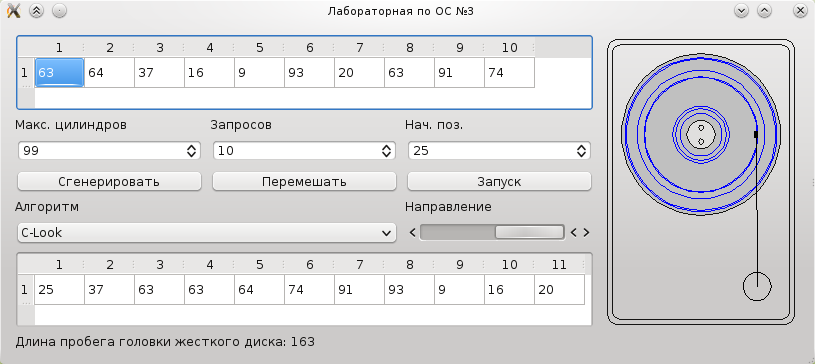
\includegraphics[width=150mm]{ioshed.png}


\end{document}
